\documentclass{bredele}
\usepackage{xcolor,colortbl}
\definecolor{blue}{RGB}{101,133,207}
\hypersetup{
colorlinks=true, %colorise les liens
breaklinks=true, %permet le retour à la ligne dans les liens trop longs
urlcolor= blue, %couleur des hyperliens
linkcolor= blue, %couleur des liens internes
citecolor=blue,    %couleur des liens de citations
bookmarksopen=true,
}
\makeatletter\@addtoreset{chapter}{part}\makeatother
\graphicspath{{"C://Users//LE GALL//Desktop//Nouveau dossier//"}}
\title{Rapport de stage de fin d'études}
%% REMERCIEMENTS %%

\lesoustitre{}
\discipline{Master 2 Démographie}
\jury{
\begin{description}
\item[Maître de stage~:] Loïc \textsc{Bourriquen}, Directeur d'études, AUDIAR
\item[Tuteur pédagogique~:] Philippe \textsc{Cordazzo}, Prof. des Universit\'{e}s, Unistra
\item[Lecteur~:] Nicolas \textsc{Cauchi-Duval}, Maître de Conférence, Unistra
\end{description}
}
\author{Marine Le Gall}
\date{\\\centering{28 Septembre 2017}}
\logouniversite{logo_univ} %nom du fichier
\scalelogouniversite{0.7} % mise a l'echelle de l'image (0.5=50% par exemple)
\logolabo{logo_labo}
\scalelogolabo{0.7}
\unite{\large{Institut de Démographie de l'Université de Strasbourg}}
\ecoledoc{\Large{Université de Strasbourg}}


\begin{document}
\maketitle
\clearemptydoublepage
\chapter*{Remerciements}
\thispagestyle{empty}
Je tiens à remercier l'AUDIAR de m'avoir permis d'effectuer mon stage de fin d'études.\\\\
Je remercie tout particulièrement Loïc Bourriquen de m'avoir acceptée en tant que stagiaire. J'ai grandement apprécié la confiance qu'il m'a offert, la rigueur de son travail comme sa capacité à penser les solutions, ainsi que les discussions sur des points très techniques comme des réflexions plus globales.\\\\
Un grand merci également à Isabelle de Boismenu qui m'a très facilement embarquée dans ses projets et a su prendre le relais quand il fallait.\\\\
Je suis très reconnaissante à l'égard de la direction régionale de l'INSEE Bretagne de m'avoir permis de suivre les études partenariales et particulièrement à Hervé Bovi et Isabelle Baudequin avec qui il a été très agréable d'échanger.
%%%%%%%%%%%%%%%%%%%%%%%%%%%%%%%%%%%%%%%%%%%%%%%%%%%%%%%%%%%%%%%%%%%%%%%
\\\\Bien évidemment cette expérience s'inscrit dans un cycle plus long et les enseignements reçus auprès de l'IDUS ont été fondateurs. Merci pour le dynamisme, les conseils et l'écoute que j'ai pu trouver auprès des équipes enseignantes. Et ce particulièrement à Philippe Cordazzo en tant que tuteur pédagogique durant ce stage.
\clearemptydoublepage
\frontmatter
\chapter*{Introduction}
%%%%%%%%%%%%%%%%%%%%%%%%%%%%%%%%%%%%%%%%%%%%%%%%%%%%%%%%%%%%%%%%%%%%%%%
%% PARTIE I %%
\addcontentsline{toc}{part}{Introduction}
\chaptermark{Introduction}
\begin{minipage}[top]{14cm}
% contenu de la minipage
\small{\textit{Le stage présenté a été effectué au sein de l’Agence d’Urbanisme et de Développement Intercommunal de l’Agglomération Rennaise (AUDIAR) du 23 janvier 2017 au 31 août 2017. La durée étant de 924h correspond au maximum légal autorisé et une période de carence a donc été imposée du 16 juillet au 17 août 2017. Il s’agit d’une expérience professionnelle venant conclure mon Master 2 de Démographie auprès de l’Institut de Démographie de l’Université de Strasbourg (IDUS) durant l’année universitaire 2016-2017.
\\Au document présent s'ajoute un second, complémentaire, intitulé Rapport de Stage. Des références y sont faites à travers les marqueurs \textcolor{magenta}{[\ding{89} + Figure + N°]}. \\L'ensemble des fichiers est disponible en ligne : \href{https://github.com/mlegall/GIT1}{https://github.com/mlegall/GIT1}}}
\end{minipage}
\\\\\\Avant même de découvrir les agences d’urbanisme j’avais entendu parler de cette structure puisque mon attachement au territoire rennais est établit de longue date. J’avais ainsi pu apprécier les études produites qui avaient, très tôt, retenu mon attention. La convergence des compétences alors développées durant mon cursus avec le cœur de métier porté au sein de l’AUDIAR m’ont naturellement amenée à adresser une candidature spontanée. J’entends par là l’analyse des problématiques sociétales, du dynamisme territorial et de la cohésion tant sociologique qu’économique à l’échelle locale, ainsi que l'apport de réponses à visée opérationnelle.
\\\\
Lors de ma phase de prospection j’avais alors étendu mes recherches à d’autres structures de ce même type, mais ces dernières étant focalisées sur des territoires dont la connaissance m’était bien plus limitée m’auraient, à priori, permis une appropriation moins aisée des concepts liés à l’urbanisme et l’aménagement du territoire. En effet, si j’avais pour objectif d’approfondir la dimension technique j’étais également à la recherche d’un apprentissage plus thématique venant, à mon avis, alimenter de manière conséquente la capacité d’analyse et donc la pertinence des traitements souvent quantitatifs qu’effectue le démographe.
\\\\
Les différents services de l’agence présentent tous une singularité et mon choix s’est alors porté dans la section « Démographie et Politique de la Ville » comme définie, en ce temps, dans l’organigramme. La proposition effectuée par Loïc Bourriquen, directeur d’études de cette unité, lors de nos échanges a été portée sur la contribution à la 5ème version d’un projet de \textit{Simulateur Démographique}, d’où l’intitulé \textit{ProjetV5}. L’objectif principal était l'amélioration des travaux prospectifs mêlant différentes trajectoires. Il était question de traiter à proprement parlé « que » l’aspect démographique afin d’apporter une vision plus fine mais contribuant aux autres composantes puisqu’on comprendra aisément que l’évolution du territoire ne peut faire fît des dynamiques de population. Cette dimension n’avait pas était approfondie, et d’un nombre de ménage projeté en découle un nombre d’individus à travers un coefficient multiplicateur, c'est-à-dire nombre moyen de personne par ménage. Cette méthodologie permet alors d’avoir en tête des ordres de grandeur, ce qui est essentiel pour quantifier dans les grandes lignes de la demande en logement par exemple. Cependant l’offre en logements et équipements, dans un contexte de fort accroissement démographique, passé et pré-supposément à venir,  n’a de sens que si elle s’adapte à la caractérisation  de cette dernière. Quid des aménagements pour accueillir les jeunes enfants ? Du nombre de personnes âgées à prendre en charge dans 10, 15, 20 ans? Quels types de logements construire : 1, 2, 3 chambre(s) ? La mission du stage était donc définie pour venir apporter un éclairage à ce genre  de problématiques qu’aucune autre structure ne fournit à l’échelle de Rennes Métropole.
\\\\
Au-delà des aspects de réflexion, les réponses apportées sont d’ordre technique et l’appareillage mis en place s’inscrit d’une tradition d’ingénierie statistique, d’autant plus que Loïc Bourriquen qui a porté ce projet maitrise particulièrement ces méthodes. En ce sens ce stage correspond tout à fait au métier de démographe puisqu’il combine un aspect analytique mais trouve ses réponses dans le traitement de données ce qui le distingue du travail de l’aménageur, du sociologue mais également de l’informaticien. L’exercice prospectif, et non prédictif, apparaît plus que délicat tant les facteurs exogènes sont nombreux. De plus, ces travaux s’adressent à un public divers (élu communal, élu métropolitain, aménageur etc.) dont les pouvoirs décisionnels influent réciproquement sur ces dernières. L’AUDIAR se donne également pour mission la concertation. C’est pourquoi le simulateur doit être capable de proposer différents hypothèses et de montrer l’impact des choix potentiels. Cela se traduit alors par la mise en œuvre d'une interface dynamique intégrant plusieurs curseurs de variation. La mission était donc de venir intégrer les travaux prospectifs démographiques affinés dans cet environnement.
\\\\
Afin de contextualiser les éléments de lecture à venir, il faut avoir en tête qu’une seconde étude, initialement secondaire mais complémentaire, a pris plus d’importance que prévu durant cette période de stage. La seconde mission qui sera alors présentée a été la contribution aux études partenariales entre l’AUDIAR et l’INSEE\footnote{Institut National des Statistiques et Etudes Economiques} portant en l’occurrence sur les migrations résidentielles grâce à la mise à disposition de nouvelles sources de données, le fichier FiDéli.
\\\\
Le déroulement du projet principal a été altéré par des absences de plus en plus fréquentes de mon maître de stage. De ce fait les éléments présentés sont plus théoriques que pratiques et le poids de la démarche l’emporte sur la diffusion de résultats, puisque la production n'est pas opérationnelle. Ainsi, les enseignements de ce stage ont été très riches et dépassent le cadre strictement pédagogique.
\clearemptydoublepage
\shorttableofcontents{Sommaire}{0}
\clearemptydoublepage
\mainmatter % Ne pas oublier, avec \frontmatter et \backmatter
%%	PARTIE 1 %%%
\part[Structure d'accueil]{Présentation de la structure d'accueil}
\chapter[Les agences d'urbanisme]{Les agences d'urbanisme}
\section{Fonctionnement général}
Les agences d’urbanisme ont un statut à part puisqu’elles sont homologuées comme association de droit privé. Rattachées à un territoire, leur périmètre d’action est limité et elles ont pour but de travailler aux échelles intra et intercommunales. Ces services d’intérêt général sont souvent détachés mais en grande partie financés par les instances de politique locale. Elles ont pour vocation d’être garant de la cohésion du territoire d’action en optimisant les décisions et trajectoires entreprises à travers l’ensemble des politiques publiques. Les principaux champs d’action relèvent des questions d’habitat, de transport, d’environnement, des aménagements urbains et paysagers tout en intégrant le dynamisme économique. En ce sens, leur travail est centré sur l’observation, l’anticipation et le conseil, permettant à la fois aux « décideurs » d’établir leurs directives puis, par répercussion, d’ériger les feuilles de route et contraintes applicables à l’action des « bâtisseurs » pour un territoire spécifique [Cf. Figure 1.1]. L’expertise des agences sur les problématiques urbaines leur permet mener les instances de concertation entre les acteurs du développement en y intégrant de temps à autre les principaux intéressés, c'est-à-dire les habitants des zones en question.
\begin{figure}
\begin{center}
\includegraphics[width=\textwidth]{schema_AGURBA.png}
\end{center}
\caption{Schéma explicatif du positionnement de l'agence d'urbanisme à l'échelle locale}
\end{figure}
\newpage
\section{Réseau national}
L’ensemble des agences d’urbanismes sont fédérées dans un réseau national, la FNAU\footnote{Fédération Nationale des Agences d'Urbanisme}. Il s’agit d’avantage d’un espace d’échanges et de dialogues que de projets directement opérationnels. En effet, si chaque territoire est spécifique sur bien des aspects, les questions de développement local se recoupent. Ainsi on retrouve un espace de concertation à travers lequel sont organisés des publications communes, des séminaires thématiques pour les chargés d’études mais où s’établit également un contact avec les réseaux nationaux des acteurs partenaires et les services ministériels. Actuellement on recense une cinquantaine d’agences d’urbanisme en France métropolitaine mais également dans les territoires ultra-marins. Les intercommunalités présentent des tailles variables et une grande partie d’entre elles ne sont pas enregistrées en tant que métropoles.
\section{Coopérations intermédiaires}
Les grandes intercommunalités prennent de plus en plus de poids mais ne peuvent pour autant être totalement autonomes. C’est pourquoi les agences s’associent souvent par réseau de proximité, en témoignent les différentes coopérations actuellement en place [Cf.Figure 1.2]. L’échelle régionale fait sens avec des problématiques économiques partagées et correspond également à un territoire de décision politique couverts par les conseils régionaux, également responsables d'aménagements territoriaux.
\\\\La région Bretagne compte à elle seule 4 agences, couvrant des périmètres élargis. Le partenariat de ces dernières leur permet d’avoir des réflexions communes, puisque ces sous-systèmes sont interdépendants. Par exemple, le projet de la nouvelle ligne à haute vitesse a un effet immédiat sur Rennes mais aura des répercussions certaines sur l'ensemble de la région de manière directe ou par ricochet. Les travaux prospectifs des uns ont un impact direct sur les décisions à prendre de l’autre. Cela permet donc d’envisager un équilibre un peu plus global garantissant une meilleure dynamique des territoires. L’élargissement permet également de couvrir au mieux les espaces biens moins urbanisés.
\\\\Le développement d’outils communs se traduit par exemple par  des bases de données mutualisées.
\begin{figure}
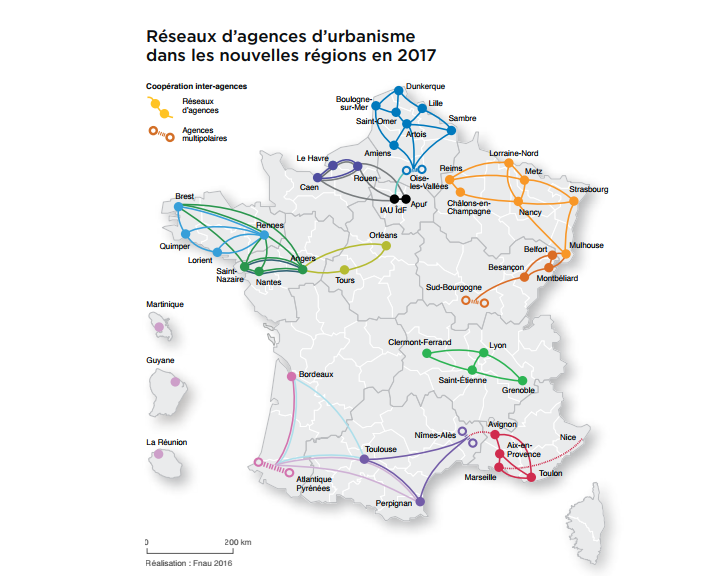
\includegraphics[width=\textwidth]{AgenceFNAU.png}
\caption{Agences d'urbanisme appartenant au réseau FNAU en 2017 et leurs différentes coopérations intermédiaires}
\begin{flushright}
\Source{Source : FNAU}
\end{flushright}
\end{figure}
\chapter[L'AUDIAR \& son environnement]{L'AUDIAR \& son environnement}
\section{Le territoire}
\subsection{Les géographies}
La notion de périmètre d’action est à définir sans cesse. Si on se contente de lire dans l’appellation de l’agence, l’intercommunalité se traduit désormais par Rennes Métropole. Depuis janvier 2017 cette entité se partage entre 43 communes hétérogènes liées par un pacte à dimension politique évoluant au fil du temps. Or les dynamiques ne se cantonnent pas à ces limites et de fait le territoire d'observation est élargi, souvent au département. De plus les bassins de vie avoisinants, au sens large, ne détiennent pas tous une agence d'urbanisme et font parfois appel aux services de l'AUDIAR pour l'élaboration de schéma directif d'urbanisme.
\\\\L’échelle départementale est celle qui délimite au mieux les principales frontières. Pour autant, le pays de St Malo le long du littoral nord ne détient pas d’agence d’urbanisme .
Il sera donc précisé constamment de quel système il est question.
\subsection{Forme urbaine actuelle}
L’aire urbaine de Rennes est caractérisée par un fort étalement avec une densité relativement faible. Les alentours sont principalement composés de campagne et il n’existe pas de limite physique ou administrative. De plus, la position de la capitale bretonne aux portes de la région la place au milieu d’un carrefour et non d’un passage, ce qui a eu pour conséquence un développement routier en étoile. De fait, les zones d’habitation ont pu aisément proliférer sans perdre une connexion avec les pôles d’emploi et autres zones d’activité. Les seuls quartiers faisant exception ont été construits dans la ville centre dans les années 1960 pour répondre à des besoins d'urgence et d'extension rapide du parc immobilier. 

\subsection{Les dynamiques passées}
Rennes est une ville de province et a principalement un rayonnement national. Actuellement, l’aire urbaine représente la 11ème en termes d’habitants avec 
Rennes est une ville administrative. Plusieurs activité viennent modeler le territoire : les pôles universitaires portent nettement le dynamisme et chaque année près de 50 000 étudiants s'accaparent la ville\footnote{\href{http://www.audiar.org/sites/default/files/documents/observatoires/obs_universites_rennaises_poids_eco_web_0.pdf}{Le poids économiques des universités rennaises, AUDIAR, novembre 2016}}. Si ces derniers engendrent beaucoup d'arrivées, la rotation est conséquente car les départs sont également importants dès lors que les études se terminent. Le nord est caractérisé par la présence d'un technopole important, avec bons nombres d'entreprises d'ingénierie, ainsi que des cliniques privées.  Le sud était lui plus ouvrier, avec les usines de Peugeot-Citroën qui ont longtemps était un emblème far. Dans l'ensemble, le chômage est moins élevé que dans le reste du pays, notamment car le territoire a été moins exposé à la désindustrialisation que d'autres endroits, les secteurs d'activité étant centrés sur les activités agricoles, de service ou bons nombres d'emplois administatrifs. Par ailleurs, si dans l'ensemble la Métropole Rennaise est moins exposée à la pauvreté que ses homologues, il existe de fortes disparités inter-communales, et en particulier dans la ville centre\footnote{\href{https://www.insee.fr/fr/statistiques/fichier/version-html/2511239/br_ina_48.pdf}{Mixité sociale et taux de pauvreté relativement faible dans Rennes Métropole, INSEE-AUDIAR, Insee Analyse Bretagne, n°48, décembre 2016}}.
\\\\Le dynamisme démographique a connu une progression constante tout à fait remarquable depuis les années 1960 en atteignant près du double ses effectifs [Cf. Figure 2.1]. En revanche, comme dans la majeure partie du pays, le nombre de ménage augmente d'autant plus vite que celui des individus, témoignant d'une baisse considérable de la taille des ménages. Cet accroissement de population a été suivi de près par l'élargissement du parc immobilier, en gardant un taux de vacance stable et restreint. On peut alors se poser la question, à posteriori, de l'effet limitant qu'a pu avoir la taille de cette offre de logement.
\\\\Les structures par âge, mais également par ménage sont très variables selon la zone d'habitation[Cf.Figure 2.2]. La ville centre concentre la majeure partie des jeunes adultes, bien souvent étudiants, quand l'aire urbaine témoigne de structures mêlant enfants et adultes, mettant en avant des structures de ménages plus familiales. Ces différentes logiques seront détaillées dans un second temps, et font l'objet centrale de la mission sur les migrations résidentielles.
\begin{figure}
\centering
\includegraphics[width=\textwidth]{dynamiques.png}
\caption{Dynamiques observées depuis les années 1960 dans l'aire urbaine de Rennes, selon l'unité statistique}
\begin{flushright}
\Source{Source : Insee, Recensement principal}
\end{flushright}
\label{Dynamiques passées}
\end{figure}
\begin{figure}
\centering
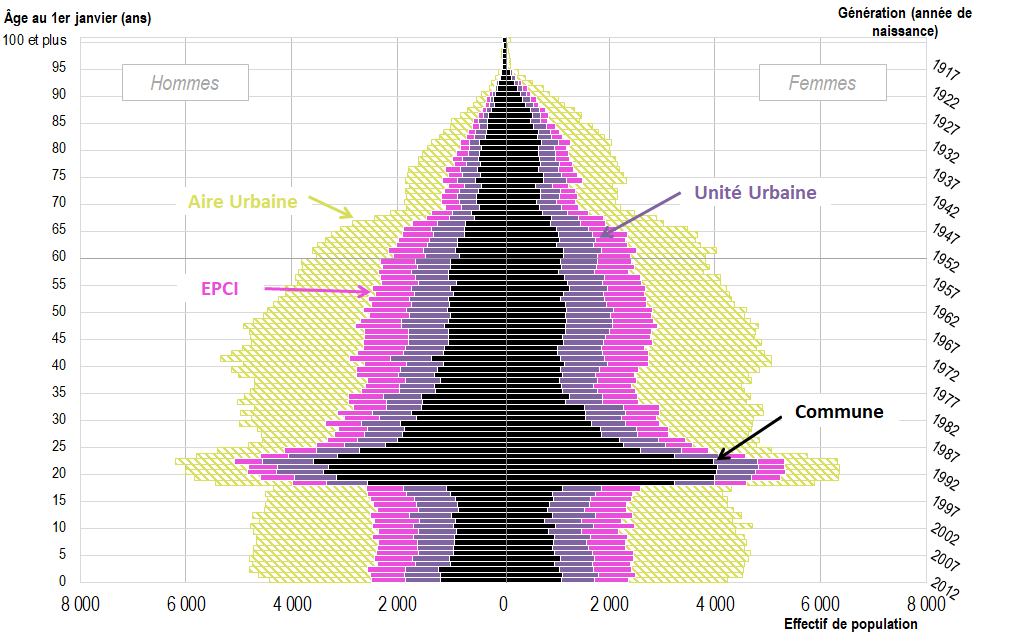
\includegraphics[width=17cm]{pyra.png}
\caption{Stucture par âge et sexe selon les différents zonages d'habitation en 2013 pour le territoire rennais}
\begin{flushright}
\source{Source : Insee, Recensement principal 2013}
\end{flushright}
\boitesimple{\small{Les dénominations sont issues du découpage défini par l'INSEE, afin de donner une idée des grands équilibres dans le territoire rennais au sens large. Les niveaux sont inclus les uns dans les autres, c'est à dire que l'aire urbaine englobe tous les niveaux inférieurs, tels que :\\
\begin{itemize}
	\item \textbf{Commune }: La commune est la plus petite subdivision administrative française, \textit{ici, Rennes}
	\item \textbf{Unité urbaine }:La notion d'unité urbaine repose sur la continuité du bâti et le nombre d'habitants. On appelle unité urbaine une commune ou un ensemble de communes présentant une zone de  bâti continu (pas de coupure de plus de 200 mètres entre deux constructions) qui compte au moins 2 000 habitants.
	\item \textbf{ECPI :} Les établissements publics de coopération intercommunale (EPCI) sont des regroupements de communes ayant pour objet l'élaboration de « projets communs de développement au sein de périmètres de solidarité », \textit{ici, Rennes Métropole}
	\item \textbf{Aire urbaine}: Une aire urbaine ou « grande aire urbaine » est un ensemble de communes, d'un seul tenant et sans enclave, constitué par un pôle urbain (unité urbaine) de plus de 10 000 emplois, et par des communes rurales ou unités urbaines (couronne périurbaine) dont au moins 40 \% de la population résidente ayant un emploi travaille dans le pôle ou dans des communes attirées par celui-ci.
\end{itemize}
}}
\end{figure}
\newpage
\subsection{Les politiques locales}
La politique du choc de l’offre a été décidée il y a une dizaine d’année à la suite d’importantes tensions sur le marché du logement. Aujourd’hui, l’agglomération rennaise ne fait pas partie des marchés immobiliers en tension comme le met en avant la loi ALUR\footnote{Accès au Logement et Urbanisme Rénové}(2014) à travers son dispositif d'encadrement durable des loyers, quand les agglomérations de cette envergure sont généralement concernées; cela exprime une offre de logement désormais conséquente malgré une demande soutenue.
\\\\Rennes se veut solidaire, et dans un soucis de plus grande mixité sociale il vient d’être mis en place la politique de loyer unique dans les logements sociaux, afin que les personnes les moins favorisées puissent avoir une trajectoire résidentielle la moins subie possible. Conjointement, la localisation de ces logements a été rendue plus homogène, c'est-à-dire que les communes hors noyau urbain sont davantage impliquées dans le processus. Les quartiers prioritaires de la ville concentrant une grande part des ménages concernés étaient au nombre de quatre et se situent tous intra-muros.
\\\\Dans ce même plan d’urbanisme la préservation des zones rurales apparait comme un élément crucial. Ainsi, la redensification du cœur de métropole à travers la conversion de maison en immeuble par exemple est actuellement en cours, la morphologie urbaine se modifie considérablement.
\\\\L’impact de ces mesures est donc à prendre en compte mais ces expérimentations viennent remodeler et donc intégrer un peu plus d’incertitude dans les travaux prospectifs.
\subsection{Projets à venir}
Au-delà des décisions locales, on retrouve d’autres projets ayant un potentiel dynamique. Ils n’ont pas nécessairement l’ambition de mettre Rennes en orbite mais lui permettront sûrement de tirer son épingle du jeu à l’heure de la métropolisation.
\\\\Le principal d’entre eux vient d’être inauguré, il s’agit de la ligne à très haute vitesse connectant Rennes à 1h25 de Paris. Entre réel potentiel d’attractivité et sur-communication les discussions vont bon train, mais plusieurs scénarios sont envisageables. Le scénario 'idéal' imagine  une localisation importantes de nouvelles entreprises engendrant l’arrivée de nouveaux travailleurs, pour la plus part très qualifiés. Un seconde effet pourrait être lié à la grande mobilité des catégories aisée à travers le déménagement de ménages dont un actif au moins détient une activité professionnelle localisée dans la capitale, par exemple. Un autre prisme de lecture met en avant une simple mise à jour du réseau permettant à Rennes et la région de rester dans la course puisque les travaux ont été entrepris dans plusieurs partie du pays. Dans une version plus pessimiste, les mobilités ne deviennent que sélectives de par les tarifs en augmentation et donc dans une certaine mesure un scénario avec effet limitant, en particulier sur les déplacements quotidiens.
\\\\L’historique des universités rennaises n’a pas lieu d’être ici retracé cependant la fusion des deux principales entités devraient avoir lieu dans les années à venir et les ambitions de mener ces pôles à une dimension internationale.  Cela contribuerait à attirer de nombreux étudiants et des actifs hautement qualifiés ce qui constitue sans nul doute un objectif politique afin de contribuer au bon dynamisme économique.
\\\\De même, le centre hospitalier de Pontchaillou va entamer une grand recomposition, l’amenant à devenir un pôle de santé encore plus conséquent.
\\\\D’autres secteurs économiques stratégiques se développent comme le secteurs des nouvelles technologies et également de la défense.
\\\\La vitalité intrinsèque du territoire elle se traduit par la construction d’une nouvelle ligne de métro traçant une diagonale opposée à la première, permettant ainsi de quadriller la ville et de mieux connecter des quartiers plus enclavés. De même, une prison va être implantée et le projet d’une aréna est en cours de consultation.
Les programmes de rénovation urbaine se font dans le long terme, aussi bien dans les bâtiments historiques avec des requalifications dans le cadre dune OPAH-RU\footnote{Opération Programmée d'Amélioration de l'Habitat et de Renouvellement Urbain}, portée conjointement par la métropole et l'ANAH\footnote{Agence Nationale de l'Habitat}. Cette perspective est également suivie pour des habitats plus récents, en particulier dans le cadre du NPNRU\footnote{Nouveau Programme National de Rénovation Urbaine}, en améliorant le cadre de vie de quartiers caractérisés d'intérêt national principalement constitués de grands ensembles.
\section{Eléments structurels de l'agence}
\subsection{Organisation hiérarchique & évolution}
L’organigramme de janvier 2017 a connu des évolutions au cours des derniers mois [Cf. Figures 2.3 et 2.4]. Il existe cependant des éléments invariants. 
\\\\La présidence de l’AUDIAR est héritée de la fonction de président de Rennes Métropole. Cependant le poste de directeur est lui occupé par une personne dédiée à plein temps. 
\\\\La restructuration s’est faite d’une part par l’intégration de Conseil de Développement, avec 3 nouveaux salariés ainsi que 2 départs en retraite ayant donné lieu à 1 remplacement. Ces mouvements ont été accompagnés par une restructuration progressive du fonctionnement sur le cœur de métier plus que les emplois de fonction dites support. Auparavant les équipes de chargés d’études étaient rattachées à des directeurs d’études sur des problématiques spécifiques. Désormais, ces problématiques n’apparaissent plus en tant que telles et de fait chacun est amené à devenir plus polyvalent. Des postes dits de support viennent également renforcer le travail d’études à travers par exemple un service de reprographie, d’infographie ou de comptabilité , puisque très peu de tâches sont externalisées.
\begin{figure}[b] \centering
\includegraphics[width=12cm]{organigramme1.png}
\caption{Organigramme de l'AUDIAR au premier trimestre 2017}
\begin{flushright}
\source{Source : AUDIAR}
\end{flushright}
\end{figure}
\begin{figure} \centering
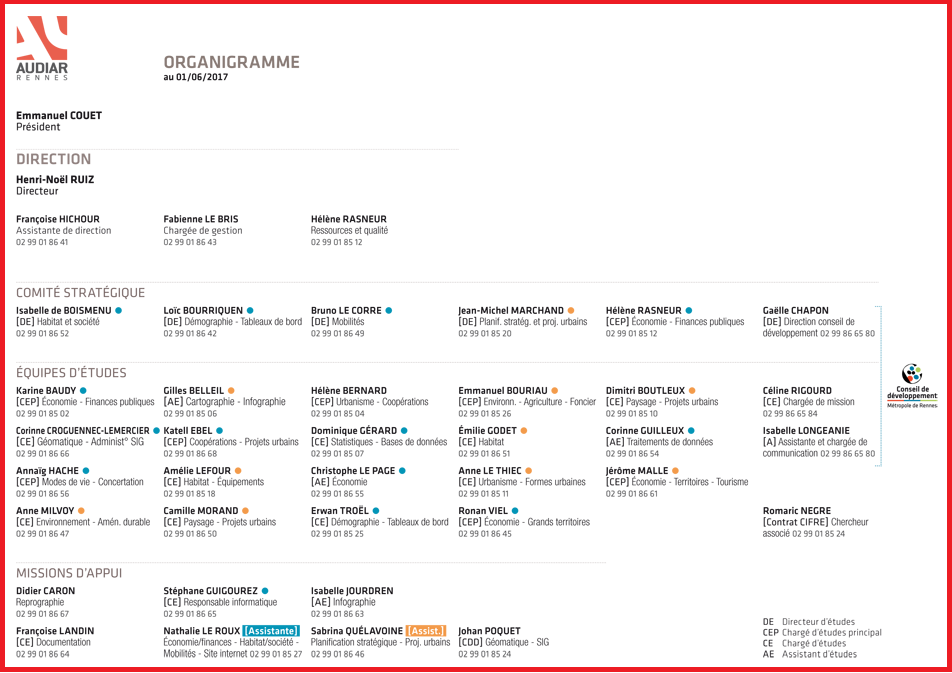
\includegraphics[width=12cm]{organigramme2.png}
\caption{Organigramme de l'AUDIAR à partir de mars 2017}
\begin{flushright}
\source{Source : AUDIAR}
\end{flushright}
\end{figure}
\subsection{Contexte}
\subsubsection{Décentralisation}
Si l'effet n’est pas exclusif à l’AUDIAR, la période se prête à une réduction des moyens alloués du fait de coupes budgétaires publiques. C’est pourquoi l’objectif de réduire le nombre de personnes en emploi est d’actualité. Cela a pour conséquence une surcharge de travail pour certains postes mais également un recentrage des priorités et de fait des thématiques laissées de côtés.
\subsubsection{Electoral}
La période couverte par le stage a été ponctuée de nombreuses échéances électorales principalement nationales mais laissant entrevoir une possible recomposition des pouvoirs en place. Rennes et ses alentours sont ancrés depuis des années dans une tradition socialiste. L’actuel président de l’AUDIAR a donc mis son poste en jeu à travers une candidature aux élections législatives. Par anticipation, il avait été envisagé une succession à ce poste laissant entrevoir de possibles réorientations des missions, mais ce dernier a rapidement été coupé dans son élan. De fait, après une période de suspension, les orientations ont repris leur cours courant juin.
\clearemptydoublepage
%%%%%%%%%%%%%%%%%%%%%%%%%%%%%%%%%%%%%%%%%%%%%%%%%%%%%%%%%%%%%%%%%%%%%%%#############
\part[Missions de stage]{Présentation des missions de stage}
\chapter[Simulateur Démographique]{Simulateur Démographique}
\section{Cadre de travail}
\subsection{Enjeux liés au projet}
Les travaux entrepris durant ce stage viennent s’inscrire dans un projet de longue date et ont pour but de le consolider. Le socle préexistant a connu plusieurs volets d’évolution et contient différents niveaux d’informations prospectives. Le périmètre systémique est celui de Rennes Métropole, qui correspond à un territoire particulier de décision et d’action politique, mais également de financement. Ainsi les résultats issus du simulateur donnent une vue d’ensemble sur le périmètre qui se doit d'être cohérent, mais également un niveau plus fin, qui est celui de la commune. La localisation fine permet donc de s'adresser à chaque unité décisionelle et constitue un élément intéressant pour dialoguer avec les différents acteurs impliqués.
\\\\
Un des objectifs principaux de cet objet est non pas la prédiction mais plutôt de l’aide à la décision à travers une prise de conscience de l’impact que peut avoir telle ou telle décision concernant principalement les orientations d’aménagement. La version dite « cliente » se présente donc sous forme d’interface interactive où il est possible de faire varier quantitativement les différentes hypothèses de projection[Cf. Figure 1.1]. Les résultats et seuils maximaux apparaissent alors de manière chiffrée mais également sous forme graphique ce qui peut permettre une prise de conscience plus aisée qu'un ensemble de tableaux de données pour qui n'est pas familier.
\\\\
Différentes trajectoires sont modélisées et on peut ainsi constater les niveaux nécessaires de chacune qui amèneraient à un point d’équilibre désiré, et par opposition, les éventuelles divergences.
\\\\
Une première trajectoire est établit sur le nombre de \textit{logements} en prévision à raison du trimestre. Ces décisions sont en partie déjà prises, mais des ajustements peuvent toutefois être opérés par les aménageurs à posteriori, tant que les lots ne sont pas réellement en projet. La trajectoire est donc relativement fiable et facile à modéliser par commune.
\\\\
La seconde en découle, et correspond aux \textit{consommations d’espace}. Chaque commune détient sur son territoire une surface qu’elle peut urbaniser, définie par les plans d’urbanismes qui répondent à différents critères mais surtout à une cohérence territoriale. La confrontation des deux trajectoires permet donc de reconsidérer la faisabilité des logements par la contrainte de ces espaces, ou du moins le type d’habitation possiblement constructibles. Cette première partie peut être considérée comme une modélisation de l’offre potentielle de logements.
\\\\
Ensuite, l’intégration des effectifs projetés de population est faite à travers une autre trajectoire, celle des \textit{ménages}. Ces anticipations sont faites à partir de travaux opérés avec l’INSEE avec le choix de l’hypothèse centrale, intitulée " au fil de l'eau ajustée\footnote{\href{https://www.insee.fr/fr/statistiques/fichier/1291303/OCTANA43.pdf}{Les populations de la Bretagne à l'horizon 2040 : cinq scenarios alternatifs, INSEE Bretagne, Octant Analyse, n°43, fév. 2013}}". Les attributions aux communes sont faites de manière dérivée, c'est-à-dire via l’attribution d’un poids relatif correspondant à une attractivité potentielle et au poids initial de la commune. Si l’effectif global projeté est fixe, le nombre de ménage est variable. Cette déclinaison est intégrée à travers le nombre moyen de personnes par ménage, indicé \textit{k}. Il est donc possible d’influer sur la trajectoire en jouant avec cette variable, avec pour hypothèse sous-jacente que le desserrement  de la taille des ménages peut être plus ou moins conséquent. Cette approche présente un intérêt certain puisque la tendance décroissante est avérée et la plupart des travaux prospectifs abondent dans ce sens. Les résultats livrent donc des tendances lourdes et la marge d’erreur est faible bien qu'elle soit malgré tout dépendante des projections initiales.
\\\\Pour autant, les coefficients \textit{k} peuvent varier d’une commune à l’autre, et au-delà des modes de vie l’impact des cycles de vie sont importants, notamment à moyen terme. Par exemple, des couples de personnes âgées connaissent un risque non négligeable de faire face au veuvage, des familles avec enfants majeurs risquent également de connaitre des décohabitations. A contrario les couples ayant des enfants en bas âges auront une structure de ménage relativement stable sur les 20 prochaines années. C’est pourquoi les structures de population actuelles définissent déjà une grande partie de ce \textit{k} de demain, et les variations inter-communales seront probablement marquées. Les communes périphériques en particulier n’en sont pas au même endroit dans leur histoire, les livraisons de logements n’étant pas intervenus au même moment . De plus les sociologies des communes ne sont pas les mêmes. Le travail prospectif peut toutefois être fait au cas par cas de manière annexe et la réponse globale demeurer satisfaisante.
\\\\De manière générale, il semble ainsi difficile de faire fît des tendances démographiques qui ne sont en aucun cas exogènes et, à contrario, viennent limiter ou amplifier les efforts entrepris au niveau politique du fait de leur forte inertie. Par exemple, un solde migratoire conséquent engendre une forte croissance seulement si le solde naturel n'opère pas dans le sens inverse; l'élargissement du parc de logement peut avoir comme impact d'uniquement contenir la population présente avant même de permettre l'accueil de nouveaux arrivants. Il était donc important de prendre conscience des évolutions à venir et des tendances démographiques à travers une lecture plus affinée.
\\\\L’objectif donc de ce stage est de venir superposer une trajectoire démographique à celles présentées ci-dessus. L’unité de base reste l’individu mais la consolidation en ménage est une dimension non négligeable au regard du type des objectifs de l’agence puisque c’est à ce niveau que l’offre et la demande de logement viennent se rencontrer, à la fois en termes quantitatifs mais également qualitatifs au travers des typologies de logements afin de s’adapter aux besoins des populations.
\\\\
\begin{figure}\centering
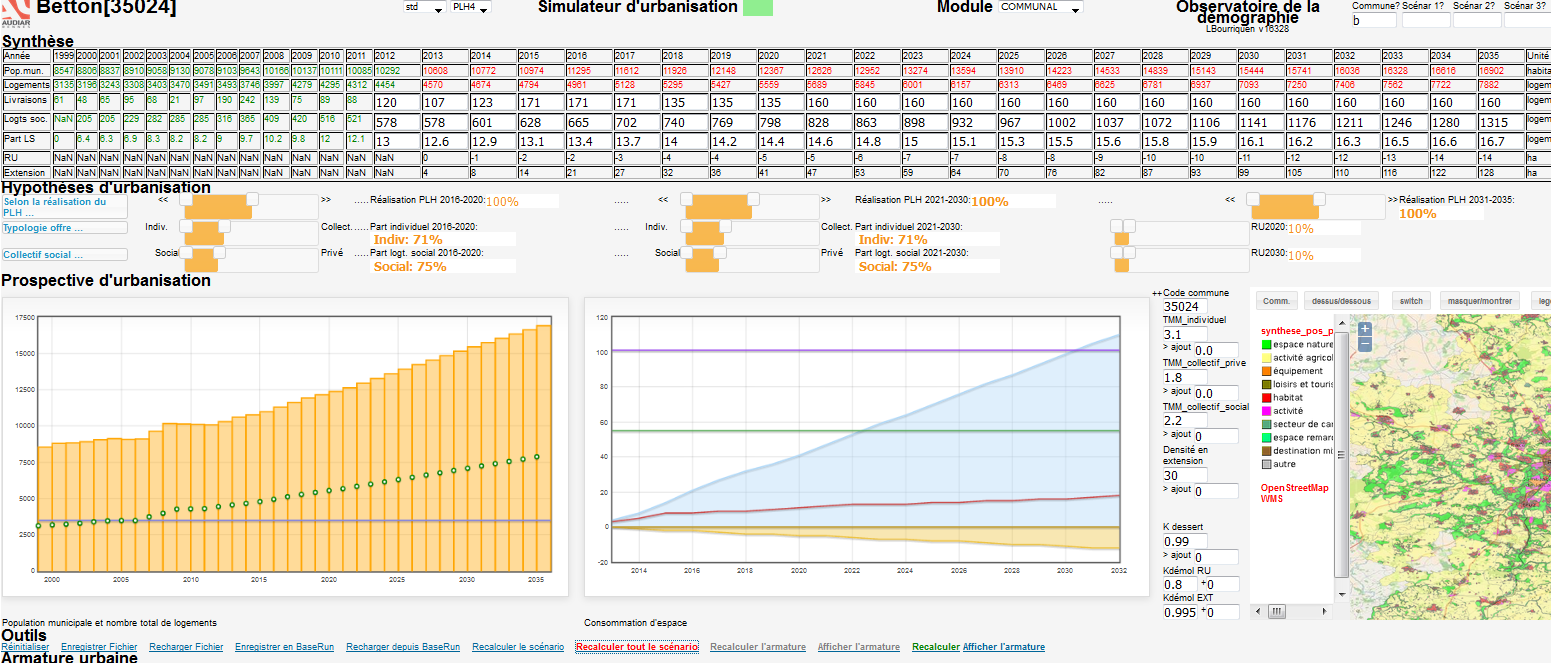
\includegraphics[width=\textwidth]{VUEV5.png}
\caption{Interface client du Simulateur Démographique}
\begin{flushright}
\source{Source: L. BOURRIQUEN, Audiar}
\end{flushright}
\end{figure}
\clearpage
\subsection{Processus de travail}
La méthode de travail, \textit{méthode en V}, mise en place dans ce projet correspond à une approche de recherche en développement [Cf. Encart]. Le but était de trouver une solution à des grands objectifs sans passer par un cheminement prédéfini. Il a donc fallu mettre en place des outils à priori et au fil de l'avancée dans le projet les réadapter à la commande et aux difficultés rencontrées. Par ailleurs, il était difficile de prévoir si l'intégralité des objectifs seraient atteints dans le temps imparti.
\\\\Afin de définir un cadre, le projet comportait des grandes phases structurantes : 
\begin{itemize}
	\item Appropriation
	\item Réalisation
	\item Rendu final
\end{itemize}
\\\\Un plan de travail plus précis a été défini à la suite de la première phase d'appropriation pour laquelle un mois devait suffire.
\\\\
\begin{center}
\begin{minipage}{16cm}
\boitemagique{Méthode d'organisation en V}{
\begin{center}
\textit{Méthode incrémentale et itérative.}\\
\end{center}
\textbf{Itératif :} le processus de développement est appliqué plusieurs fois.
\\
\textbf{Incrémental :} chaque itération augmente la quantité d’information.
\\\\Cette conceptualisation est une amélioration du modèle en cascade, c'est-à-dire d’un enchainement des étapes de production. La différence principale est que le travail se fait en aller-retour sur les différentes étapes de production, qui permettent des améliorations et des ajustements pour une cohérence entre l’idée initiale et la production finale.
\\\\En définissant un tel cadre, les marges de manœuvre sont plus larges, l’erreur potentielle est intégrée dans la philosophie du projet il est donc possible de tenter une idée audacieuse. Cela peut permettre une plus grande qualité à travers des améliorations possibles tant que le produit n’est pas livré et également une réactivité aux problèmes découverts. 
\\\\En contrepartie, un trop grand nombre d’embuches non anticipées peut entrainer une perte de temps : dans la livraison du produit final voire même dans sa non-faisabilité.}
\end{minipage}
\end{center}
\begin{figure}\centering
\includegraphics[width=\textwidth]{methodeITER.png}
\caption{Schéma explicatif de la méthode de travail, dite Itérative}
\begin{flushright}
\source{Source : \href{https://www.irisa.fr/triskell/members/pierre-alain.muller/teaching/demarche}{P.-A. Muller, Irisa}}
\end{flushright}
\end{figure}
\newpage
\subsection{Chronologie}
La chronologie de ce projet a donc été établie en plusieurs temps : le premier mois, de fin janvier à fin février avait pour objet l'appropriation, ce qui a donc définit une première période.
De même, la contrainte en bout de chaîne était de se donner pour cap la fin du mois de juin pour terminer les réalisations à proprement parlé. Ainsi, le dernier mois devait davanatage être consacré à la mise en valeur des résultats ainsi qu'à une synthèse du travail.
\\\\L'organisation interne de la phase s'est dessinée au mois de février dans le but de mieux atteindre les objectifs fixés. Cela n'était en aucun strict mais permet principalement de se rendre compte de l'avancée des travaux [Cf. Figure 1.3]. Ces étapes internes sont relatives à la nature même du projet :
\begin{itemize}
	\item Construction d'une base de donnée
	\item Construction des hypothèses naturelles
  \item Faire naitre
	\item Faire vieillir
	\item Construction des hypothèses de migrations
	\item Générer les migrations
	\item Intégrer dans l'interface
\end{itemize}
\\\\La première partie, jusque fin mars a été tenue et par la suite le calendrier et les tâches à accomplir ont commencé à diverger du cadre initial. D'autres tâches ont pris le relais et notamment la partie d'études sur les migrations résidentielles qui n'était plus que de l'observation.
\\\\Ces éléments fixés en amont n'ont pu su résister tout au long du stage. D'une part, l'évaluation du temps nécessaire était trop courte au regard de la vitesse de travail. Car parallèlement à ces tâches, l'apprentissage des outils techniques a pris une part importante et surtout l'optimisation des temps de calculs a parfois ralenti le travail, car je n'ai pas toujours su les anticiper dans les étapes de construction antérieure.
\\\\De plus, les absences du maitre de stage ont été conséquentes. Ainsi, personne n'était en mesure de tutorer le projet et au bout d'un certain temps les erreurs se sont accumulées et les problèmes à résoudre de plus en plus conséquents.
\\\\Au total sur la période 49\% du temps réel de stage a été effectuée en présence supervisée [Cf. Figure 1.4]. Cela est gênant dans la mesure où pendant des périodes entières j'ai du travailler en autonomie totale.

\begin{figure}\centering
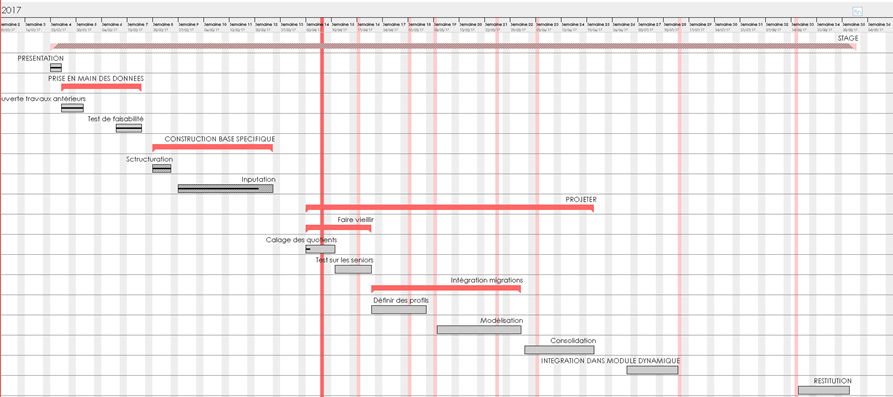
\includegraphics[width=\textwidth]{calendrierV1.png}
\caption{Calendrier des étapes de travail et objectifs établit en début de stage}
\end{figure}
\begin{figure}\centering
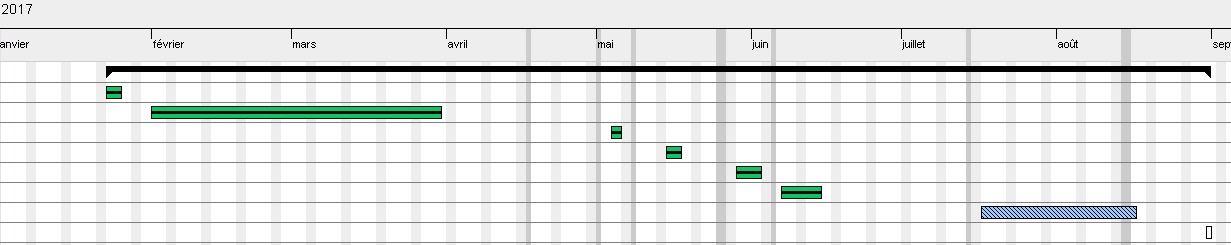
\includegraphics[width=\textwidth]{TempsPresencePartagee.png}
\caption{Calendrier des temps de présence partagée avec le maître de stage tout au long de la période de stage} \\ 
\begin{flushleft}
\textit{Vert : Présence partagée \\
Bleu : Interruption de stage comme définie en amont}
\end{flushleft}
\end{figure}
\section{Méthodologie \& mise en oeuvre}
\subsection{Appropriation}
Dans cette phase d'appropriation l'objectif était de comprendre le plus en profondeur possible les logiques des enjeux, des données, de faisabilité et devait en résulter une proposition. Les contraintes imposées étaient faibles, le coeur des données était évidemment celles du recensement sans toutefois être exclusives.
\subsubsection{Périmètres géographiques}
Une partie de cette étape a été de constater les correspondances entre les différents découpages pour se rendre compte de la faisabilité et de l'intérêt des sources. C'est pourquoi fabriquer, avec Qgis, un comparateur de géographie en superposant les différentes limites a été utile. Les nombreux découpages existant correspondent à des objectifs différents : \\
\begin{itemize}
	\item Les découpages \textit{administratifs} : Région, Département, Commune ...
	\item Les découpages \textit{politiques} : Intercommunalité, 'Pays' ...
	\item Les découpages \textit{fonctionnels} : Aire urbaine, Bassin de vie ...
	\item Les découpages \textit{statistiques} : Iris, Grand quartier, Canton Ville ...
\end{itemize}


\subsubsection{Etat des données}
Le constat établit fait ressortir que les éléments nécessaires sont disparates et qu'il serait intéressant de les combiner à travers un regroupement des données[Cf. Table1.1].\\
\renewcommand{\arraystretch}{1.5}
\begin{table}
\begin{tabular}{|p{7.5cm}|p{7.5cm}|}
 \hline 
	\multicolumn{2}{|l|}{\Large{\textit{Source}}} \\
	\hline \large{Avantages} & \large{Inconvénients}\\

	\hline \multicolumn{2}{|l|}{\Large{\textit{Fichier détails Logement}}}\\
	\hline Exhaustivité - 10 000 hab., robustesse sinon & Unité principale : Ménage, Informations indiv. agrégées \\
	Localisation à l'IRIS & Informations difficilement déchiffrable pour LPRM > 2 \\
  Informations nombreuses pour la PRM \footnote{Personne de référence du ménage} & \\
	
	\hline \multicolumn{2}{|l|}{\Large{\textit{Fichier détails Individus}}}\\
	\hline Individus regroupés en ménage & Localisation au Canton-Ville\\
  Informations pour TOUS les individus & Echantillon au quart (traitement secondaire)\\
	
	\hline \multicolumn{2}{|l|}{\Large{\textit{Fichier détails Migrations}}}\\
	\hline Lieu de départ et d'arrivée à la commune & Situation antérieure non connue\\
  Situation actuelle détaillée & Echantillon au quart (traitement secondaire)\\
\hline
 \end{tabular}
	\caption{Avantages et Inconvénients des sources données potentiellement utilisables pour le simulateur démographique}
\end{table}
\subsubsection{Fouille de données}
Les données ont des volumétries très importantes et incluent des unités statistiques qui ne méritent pas d'être présentent en permanence dans l'environnement de travail. Les données ont donc été stockées dans un environnement MySql, qui est un SGBD\footnote{Système Gestion Base de Données}. L'interface classique pour interroger ces données est phpMyAdmin et le langage de requête est le langage SQL\footnote{Structured Query Language, ou langage de requete structuree}. Cependant, la visualisation des résultats s'y fait principalement sous forme de table et très peu de figures; les procédures pour obtenir des statistiques basiques, comme des distributions, sont complexes. C'est pourquoi la création d'un script de connexion depuis R dans cette bases de données, à tables multiples, m'a permis de bénéficier de la stabilité du SGBD et des facilités de traitement du logiciel R notamment grâce à des importations de données très ciblées \textcolor{magenta}{[\ding{89} Listing 1.1, Figure 1.1]}. La phase d'appropriation a donc également consister en une familiarisation avec ces environnements.
\\\\Décortiquer les logiques de pondération m'a permis d'arriver à une solution satisfaisante, c'est à dire recombiner les avantages des sources précédentes. En effet, si lors des années de collecte les pondérations correspondent à l'inverse du taux de sondage, les années suivantes elles sont estimées par l'INSEE.
\\\\Dans la première phase d'extrapolation ces estimations suivent un coefficient qui correspond à l'évolution annuelle observée du nombre de taxes d'habitation de l'année N à l'année N+1. Le coefficient est propre à chaque unité territoriale, ici l'iris (ou bien la commune quand celle-ci ne présente pas de découpage infra). Les pondérations mises à disposition sont très précises puisque leur format est un nombre réel composé de 12 décimales.
\\\\La logique est similaire pour l'interpolation, puisque les pondérations sont cette fois ci déduite selon l'hypothèse de linéarité entre le dernier niveau d'effectif estimé et les nouvelles données collectées, étant donné le décalage entre la livraison des données et la collecte.
\\\\Les pondérations sont uniformes à l'unité territoriale, quelque soit le type de ménage ou les caractéristiques individuelles. Les seules pondérations divergentes sont celles des individus hors-ménage, puisqu'ils connaissent des méthodes d'estimation non-issues des taxes d'habitation. De plus, l'intégralité des ménages et personnes recensées restent dans les bases de données jusqu'à la nouvelle collecte, seule la pondération permet l'ajustement macroscopique.
\\\\Ce qu'il faut retenir dans la perspective de ce projet est qu'il est possible d'identifier les lieux d'habitation des invdividus dans le fichier détails individus mis à disposition par l'INSEE. La pondération peut être vue comme un identifiant communal. La confusion entre communes dont les identifiants pourraient être identiques est limitée, puisque le canton-ville est déjà connu dans chacune des parties et constitue donc une première condition.
\\\\Il faut toutefois prendre une précaution supplémentaire, si ces identifiants sont les mêmes entre tous les fichiers issus du recensement, il est nécessaire de l'adapter : le fichier ménage donne une liste exhaustive, et la pondération avoisine l'unité; tandis que le fichier individu est issu du traitement complémentaire et présente donc un tirage dit "au quart", la pondération avoisine donc 4. Cependant, le taux de sondage pour ce traitement complémentaire est en train d'être réduit au cinquième, et actuellement certains individus issus du fichier détails sont associés à une pondération avoisinant 5. Les deux cas coexistent donc actuellement.
\newline
\boitesimple{
	Tel que :\\
	\textit{Ts, Taux de sondage du traitement complémentaire}\\
	$a \in \left\{4;5\right\}$ \\
	$Ts = \frac{1}{a}$ \\\\
	\textit{IPONDI, Pondération individuelle dans le fichier détails individus\\
	IPONDL, Pondération logement dans le fichier détails logement}\\\\
	CV, canton-ville\\
	\textbf{Hypothèse :} Pour tout individu 
	$_i$ présent dans le fichier détails individus,\\il existe au moins un ménage $_m$ dans la table ménage,\\ tel que $IPONDL_m = _a * IPONDI_i$\\et $CV_i = CV_m$.
\\Par association, $IRIS_i = IRIS_m$}
\subsubsection{Choix de la méthodologie}
Lors des recherches, une solution semblait intéressante, il s'agissait d'un package R, MicMac\footnote{\href{Mic-Mac project}{http://www.nidi.nl/en/research/al/micmac}}, développé par un  consortium de chercheurs européens qui applique des taux correspondant aux hypothèses de projection aux individus. Afin de récuperer les éléments, j'ai établit le contact par mail avec la responsable du projet, Mme Sabine Zine, puisque le logiciel n'était pas directement disponible. Partir de ce point là aurait pu être très interessant, mais le résultat était aggloméré, la lecture et les compositions en ménages auraient été considérablement réduits. De plus, le seul moyen d'améliorer cette solution était la manipulation du programme R pour laquelle mes compétences et celles de Loïc étaient trop restreines, cette perspective était donc périlleuse.
\\\\Ainsi, il a été décidé étant donné les possibilités qu'offrait la nouvelle base, de projeter des trajectoires individuelles en générant des nombres de manière alétoire qui amèneraient à la connaissance, ou non, des évènements pour chaque unité après la confrontation de loi de probabilité associée.
\newline
\subsection{Création de la base de projection}
Les traitements sont gardés en mémoire dans des scripts dont les opérations ont été faites à travers le \textit{langage php}. Les données se situent toujours dans la base \textit{MySql}. Afin de pouvoir avoir un aperçu sur leur bonne mise en oeuvre, des indications test et messages d'erreur ont été intégrées et sont visualisées grâce à une page html sous \textit{Mozilla Firefox}\textcolor{magenta}{[\ding{89}Listing 2.1]}. Ces éléments sont reliés à travers un serveur WAMP.\\\\
\newpage
\subsubsection{Etape n°1: \Large{Dissociation}}
Cette étape a principalement permis d'alléger les données afin de se focaliser uniquement sur les éléments de travail, c'est à dire recentrer sur la structuration des individus en ménage dans le périmètre d'observation\textcolor{magenta}{[\ding{89}Listing 2.2]}.
\\\\
Pour cela les notions de \textit{ménage} et \textit{logement} ont été séparées de la base INSEE initiale. L'information est toutefois gardée en mémoire, à travers une approche relationnelle.
\begin{figure}\centering
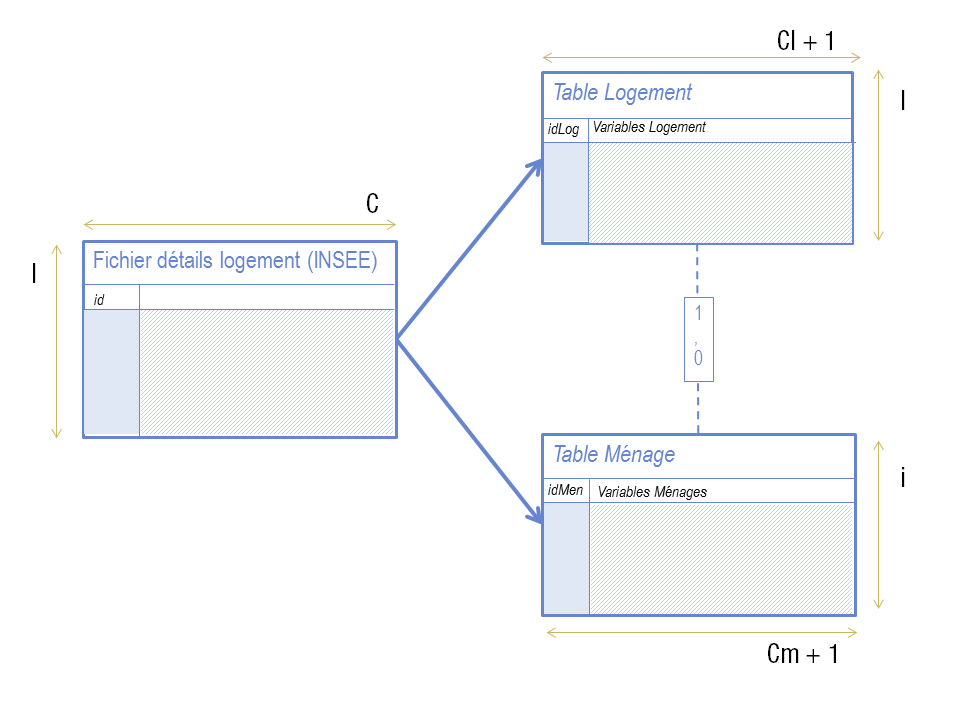
\includegraphics[width=\textwidth]{PROCESSBDD_1}
\caption{Schéma explicatif de l'étape de \textit{Dissociation}}
\boitesimple{Tel que :\\
Cl, Cm, I, i \in \mathds N \\
C = Cl + Cm ,\\
I > i 
}
\end{figure}
\newpage
\subsubsection{Etape n°2: \Large{Dislocation}}
En prenant pour point de départ l'exhaustivité de la base Ménage de l'INSEE, une nouvelle table dite individu est créée avec pour principale évolution le changement d'unité. A partir des informations contenues sur les ménages, les lignes individuelles sont générées au regard de taille de ménage contenue dans la variable INPER. Les nouveaux individus gardent l'identifiant du ménage dont ils sont issus, ce qui permet d'avoir deux niveaux de lecture\textcolor{magenta}{[\ding{89}Listing 2.3]}.\\\\
Les caracteristiques de la PRM sont nombreuses et fiables dans la source initiale, c'est pourquoi elles sont dans le même temps intégrées au premier individu généré (Age, sexe, diplôme principalement).\\\\
Si la structure est correcte au regard des informations contenues, il est toutefois nécessaire de rappeler qu'elle l'est face à l'année de collecte. Or le recensement rénové regroupe années différentes puisque les collectes sont faites par vague. Ainsi, les valeurs correspondent en moyenne à la situation de N, mais en pratique, certaines communes peuvent avoir dans cette base la situation en N-2 aussi bien qu'en N+2.\\\\
Cette exhaustivité n'est toutefois pas vérifiée pour les communes de plus de 10 000 habitants. La contrainte sera gérée lors d'une étape ultérieure et à ce stade les ménages déjà présents dans les villes concernées suivent le même traitement. \\
\begin{figure}\centering
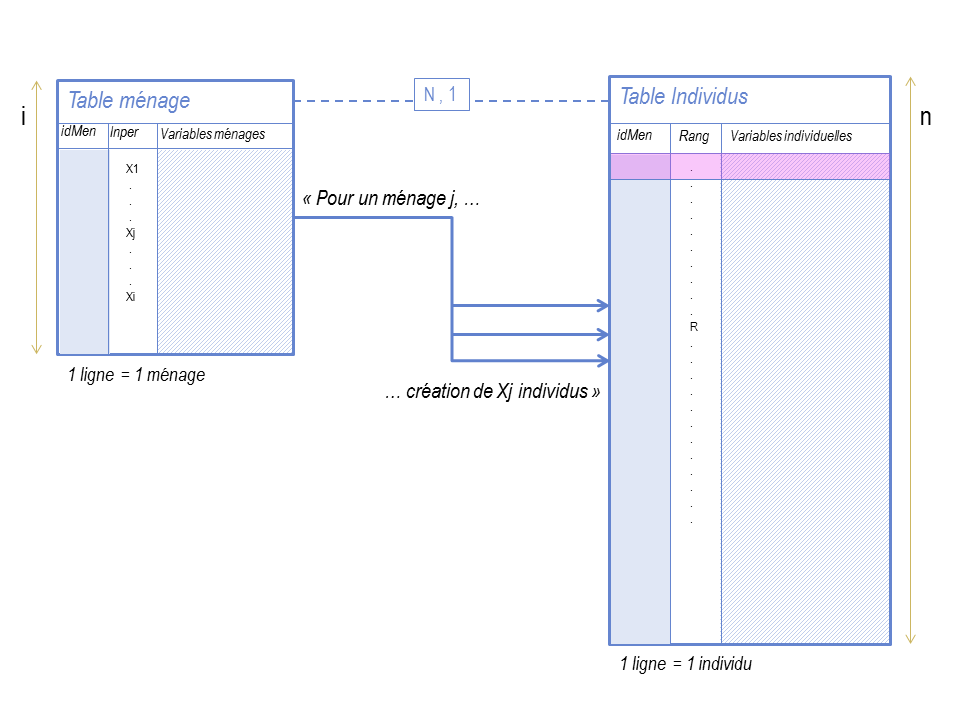
\includegraphics[width=\textwidth]{PROCESSBDD_2.png}
\caption{Schéma explicatif de l'étape de \textit{Dislocation}}
\boitesimple{Tel que :\\
$Xj, r \in \mathds N$ \\
$n = \sum_{j=1}^{i} Xj$ \\
$r < 13$
}
\end{figure}
\newpage
\subsubsection{Etape n°3: \Large{Rapprochement}}
La couverture des informations individuelles est encore partielle à ce stade. Or on sait qu'elles sont disponibles dans le fichier détails individus. C'est donc à travers le système des pondérations décrit plus haut que vont être imputées à la personne concernée. Une fois le rapprochement effectué sur la géographie, il est nécessaire de localiser le ménage correspondant et par enchainement intégrer les individus le constituant. Pour cela trois autres clefs sont créées via la concaténation des modalités sur les variables présentes de part et d'autre. La première est relative aux caracteristiques du logement, la seconde aux caracteritiques du ménages et enfin à celles de la PRM\textcolor{magenta}{[\ding{89}Listing 2.4]}.\\
\newline
Les possibilités de combinaison sont très nombreuses mais à l'échelle d'une commune il n'est pas rare de retrouver des \textit{doublons} d'autant plus que les profils des ménages gagnent en homogénéité lorsque le périmètre se restreint.
\\\\Il était donc nécessaire d'ajouter cet élément afin de ne pas insérer plusieurs fois les mêmes individus au détriment d'autres dont les identifiants centrés sur le ménage sont identiques.
\\\\Les rangs au sein du ménages ont également étaient générés de part et d'autre pour gérer au mieux cette imputation.
\\\\La couverture des informations est donc considérablement augmentée puisque désormais l'ensemble des PRM ainsi que le "quart" des individus ont leurs caracteristiques individuelles.
\begin{figure}\centering
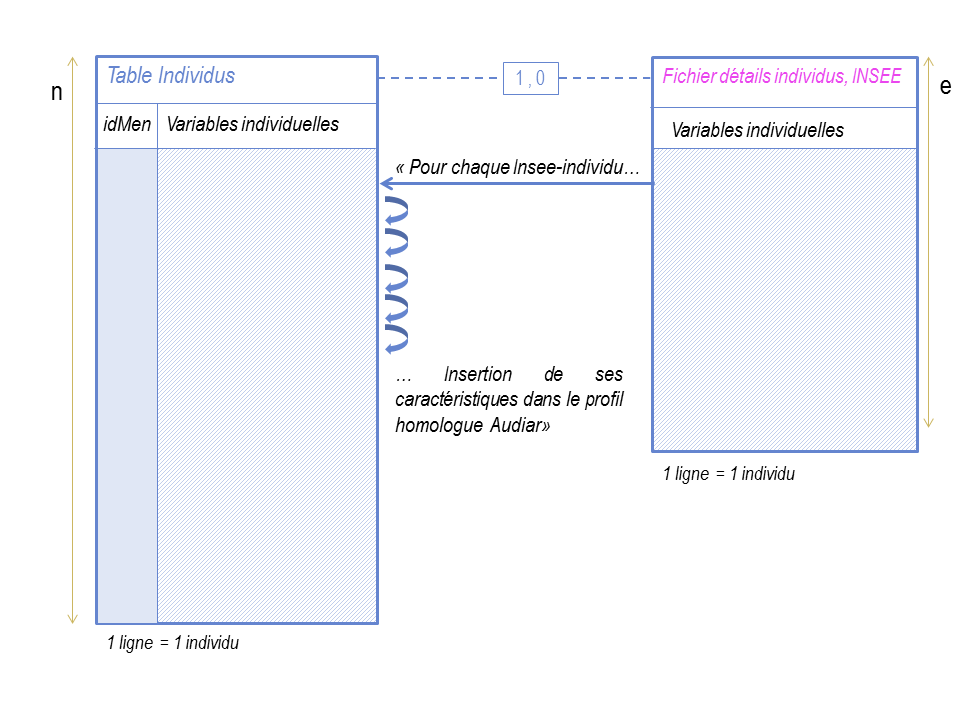
\includegraphics[width=\textwidth]{PROCESSBDD_3}
\caption{Schéma explicatif de l'étape de \textit{Rapprochement}}
\boitesimple{Tel que :\\
\large{$ \frac{n}{4}  \leq e \leq \frac{n}{5} $ }}
\end{figure}
\newpage
\subsubsection{Etape n°4: \Large{Remplissage}}
Afin de compléter cette base de données il fallait donc attribuer principalement des modalités d'âge, de sexe et de diplôme aux individus restant.\\\\
L'imputation sur le sexe a été la première phase : les personnes de rang 2 ont de facto été considérées comme des femmes. En effet, lorsque les ménages sont composés d'un couple, l'homme est quasiment toujours PRM et la femme arrive en second. La justification est plus technique que sociologique et constitue un parti-pris discutable, mais il fallait nécessairement rééquilibré ce point sans quoi le sex-ratio aurait été trop fortement déséquilibré. Pour les autres rangs, la modalité est attribuée grâce à la génération d'un nombre aléatoire : si ce dernier dépasse la probabilité, ici le sex-ratio, l'individu est une femme, sinon un homme.\\\\
Les tranches d'âges étaient dejà présentes grâce à la déduction faite sur les variables de décompte de personnes par tranche d'âge dans les ménages (INP3M , INP6M etc.). Si pour certaines tranches il était possible d'attribuer un nombre aléatoire sans grand risque d'erreur, pour d'autres, les conséquences auraient pu fausser considérablement les résultats obtenus du fait de leur amplitude (25-50 ans par exemple).\\\\
La solution la plus satisfaisante a donc été de repartir des décomptes communaux par âges quinquennaux et sexes afin de garder la meilleure cohérence possible. Toutefois, la prise en compte des individus dejà présents à été faite grâce à la soustraction de ces derniers dans la table, donnant lieu à une nouvelle, \textit{Reste à distribuer}\textcolor{magenta}{[\ding{89}Listing 2.5]}.\\\\
Les structures sont relatives à l'année de publication et donc pas nécessairement à l'année de collecte servant de base pour les communes : cela n'est pas gênant dans le cas présent puisque c'est à travers la structure relative qui va servir et non le nombre au sens strict.\\\\
A partir de ces résultats, les lois de distribution ont été recréées pour chaque commune et chaque grande tranche d'âge par sexe d'appartenir à une tranche quinquennale, toujours grâce à la comparaison du nombre aléatoire généré et la lois de distribution sous forme de probabilités, cette fois ci cumulées.\\\\
La comparaison des résultats générés et les résultats issus directement des collectes au niveau communale étaient très satisfaisants, puisqu'après plusieurs répétitions de ces calculs les pyramides des âges ne différaient que très peu. Cette phase de visualisation a été faite sur Excel.\\\\
L'attribution du niveau de diplôme n'est, quant à elle, pas faite au regard de la sociologie communale, mais vis à vis des répartitions nationales. La répartition par âge et sexe a permis de recomposer la loi de distribution de cette variable ordinale et par la suite d'attribuer le niveau correspondant à travers un nombre aléatoire  \textcolor{magenta}{[\ding{89}Figure 4.1]}.\\\\
D'autres caractéristiques auraient pu être intégrées, mais le travail est conséquent et l'intérêt pour les projections à ce niveaux n'étaient que très limité.
 
\begin{figure}[!htb]\centering
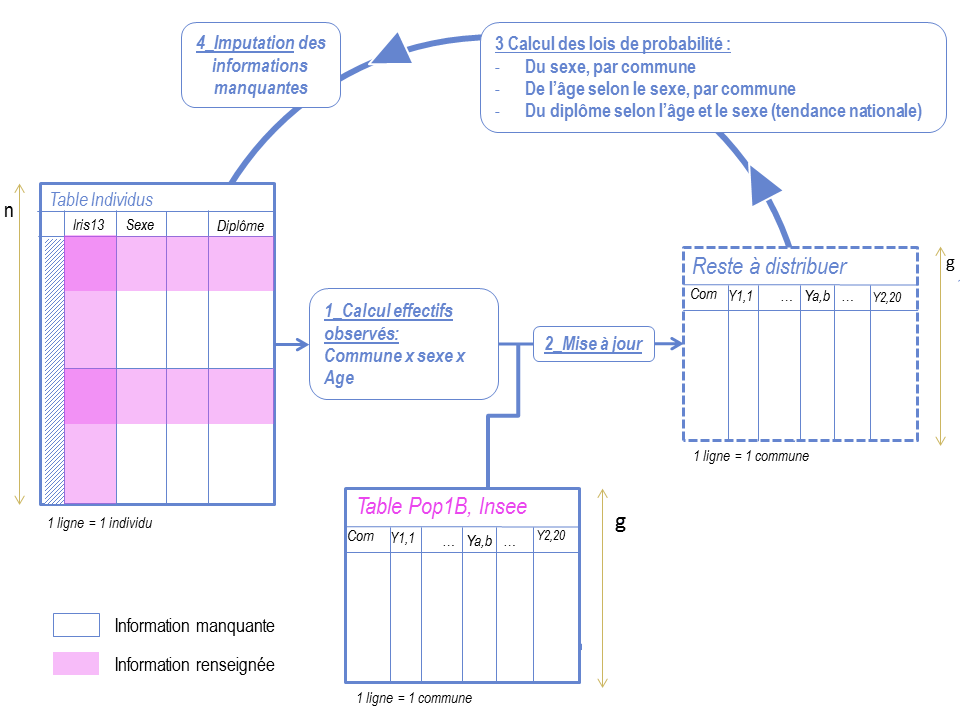
\includegraphics[width=\textwidth]{PROCESSBDD_4}
\caption{Schéma explicatif de l'étape de \textit{Remplissage}}
\boitesimple{Tel que:\\
$a \in \left\{1;2\right\}$ , sexe\\
$b \in \left\{1;20\right\}$, rang de la classe d'âge quinquennale\\
$g$, nombre de communes du périmètre\\
$Y_{a,b} \in \mathsds N$, Variable du sous-groupe Age quinquennal-sexe}
\end{figure}
\newpage
\subsubsection{Etape n°5: \Large{Projection}}
Une fois la base consolidée, l'objectif était donc de faire évoluer l'ensemble de la structure d'une année sur l'autre en anticipant les comportements éventuels des individus, mais également des ménages \textcolor{magenta}{[\ding{89}Listing 4.2]}.
\\\\En repartant de l'équation démographique générale, chaque composante a suscité un traitement.\\\\

\boitesimple{Soit \textit{t} une année donnée, \small{$
\\\\Pop_\textit{1.1.t+1} = Pop_\textit{1.1.t} + Solde Naturel_\textit{1.1.t;1.1.t+1} + Solde Migratoire_\textit{1.1.t;1.1.t+1}
\\\\Solde Migratoire_\textit{1.1.t;1.1.t+1} =  Immigrations_\textit{1.1.t;1.1.t+1} - Emigrations_\textit{1.1.t;1.1.t+1}
\\Solde Naturel_\textit{1.1.t;1.1.t+1} = Naissance_\textit{1.1.t;1.1t+1} - Décès_\textit{1.1.t;1.1.t+1}$}}
\newline
La première partie était donc de créer les bases jusqu'en \textit{t+n}.\\
Ensuite, le remplissage de ces dernières se faisaient en dupliquant les individus présents lors de l'année antérieure, plus l'ajout des potentielles nouvelles arrivées. La différence est l'état de ces derniers sur les différents points traitées. Ces états sont attribués suite à la confrontation entre un nombre généré aléatoirement par individu et la probabilité de connaitre l'évènement selon les caractéristiques socio-démographiques de l'individu concerné, comme définit dans les hypothèses de projection ci- après. En revanche, pour assurer une indépendance entre les évènements, les nombres aléatoires sont distincts d'un évènement à l'autre.\\
\newline
\\\\\textbf{1- Faire vieillir :}
\begin{flushleft}
\begin{equation}
Etat\_0101 = \left \lbrace \begin{array}{l l} 0 &  \textit{Si mort} \\
																				 1 & \textit{Si vivant en début d'année}\\
\end{array} \right
\end{equation}
\end{flushleft}
\begin{flushleft}
\begin{equation}
Etat\_3112 = \left \lbrace \begin{array}{l l} 0 & \textit{si mort} \\
$1$& \texit{si vivant en fin d'année (correspond à Etat\_0101 l'année suivante)}
\end{array} \right
\end{equation}
\end{flushleft}

\\\\Les caractéristiques du sexe et du diplôme sont gardées constantes, seul l'âge augmente d'un an lors du transfert dans la table ultérieure.
\\\\\textbf{2 - Faire naître :}
\begin{equation}
Etat\_F = \left \lbrace \begin{array}{l l} 0 &  \textit{Si n'a pas eu d'enfant durant l'année} \\
																				 1 & \textit{Si a connu une naissance (pour les femmes 15-49 ans)}\\
\end{array} \right
\end{equation}

\\\\Les ménages pour lesquels une femme a connu une naissance connaisse un ajout de ligne individu d'âge 0 dans la table suivante et l'enfant en question garde le même identifiant ménage, idMen.
\\\\\textbf{3 - Faire arriver :}
\begin{flushleft}
\begin{equation}
Etat\_I = \left \lbrace \begin{array}{l l} 0 &  \textit{Si n'est pas arrivé} \\
																				 1 & \textit{Si est entré dans RM}\\
\end{array} \right
\end{equation}

\end{flushleft}

\\\\Les immigrations sont issus des choix effectués dans la version cliente. Les profils générés sont donc tous insérés, mais leur passage d'état de 0 à 1 dépendant des paramètres entrés.
\\Par la suite, ils sont intégrés dans la base et connaissent le même traitement que les individus déjà présents. \\La logique est détaillée par la suite. Malheureusement, l'attribution à l'échelle de l'iris n'a pas été mise en place et ils sont ainsi présents dans Rennes Métropole seulement.
\\\\\textbf{4 - Faire partir :}
\begin{flushleft}
\begin{equation}
Etat\_E = \left \lbrace \begin{array}{l l} 0 &  \textit{Si reste habiter dans RM jusqu'en fin d'année} \\
																				 1 & \textit{Si déménage de RM durant l'année}\\
\end{array} \right
\end{equation}
\end{flushleft}
\\\\\\Les départs, ou émigrations, étaient censés être à l'échelle de l'individu principalement. Les logiques de décohabitation par exemple ne sont pas si compliquées à mettre en œuvre dans l'immédiat et on peut penser qu'une migration modélisée sur les personnes référentes de ménages entraine la mobilité de l'ensemble de ce dernier.
\\\\Le cadre de la partie des migrations a été pensé, partiellement anticipé, mais très peu mis en pratique.
\\\\La mobilité intra-métropolitaine, c'est à dire le changement de localisation des ménages aurait été un élément très intéressant à mettre en place mais présente une forte complexité de mise en œuvre.  Cet aspect n'a pas abouti dans le contexte du stage. Il aurait fallu établir des matrices d'échanges inter-communaux, mais la gestion de l'interdépendance semblait une tâche difficilement surmontable au regard de mes compétences. A cela se mêlent les évènements relevant des histoires de vie qui compliquent également la mise en œuvre de trajectoires claires.
\\\\Le procédé de la méthode en V a donc fait que la première phase était de travailler à un niveau macroscopique afin de valider cette échelle, et par la suite de rentrer dans des niveaux de détails plus fins et plus complexes. Cependant le contexte a fait que les éléments incorporés se focalisent principalement sur les composantes naturelles à une échelle macroscopique, et de plus sur une population fermée puisque le jeu des migrations n'a pas abouti.
\\\\La lecture des effectifs résultant de la modélisation se fait donc sur les individus ayant pour Etat\_0101 égal à 1, c'est à dire présent en début de période.
\\\\Le nombre de naissance durant l'année N se fait donc par la somme des Etat\_F égaux à 1.
\\Le nombre de décès durant l'année N se fait donc par la somme des Etat\_3112 égaux à 0.

\begin{figure}[!htb]\centering
\clearpage
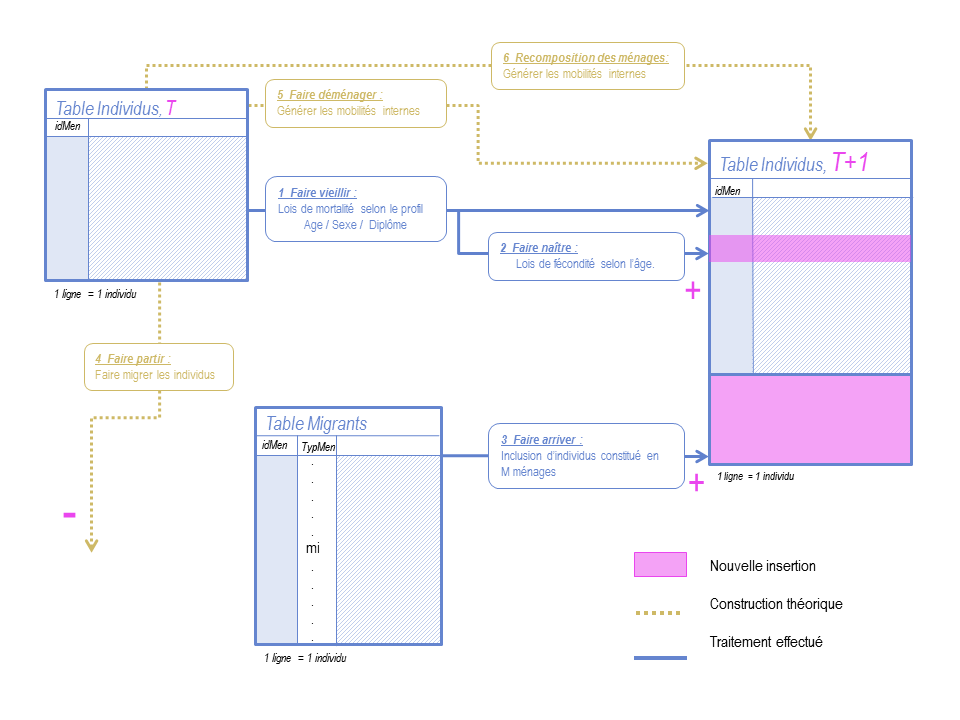
\includegraphics[width=\textwidth]{PROCESSBDD_5}
\caption{Schéma explicatif de l'étape de \textit{Projection}}
\boitesimple{Tel que:\\
$i \in \left[1;5\right]$}
\end{figure}

\newpage
\subsection{Hypothèses de projection}
\subsubsection{Fécondité}
La première approche entreprise sur cette thématique a été faite en autonomie. A travers les méthodes de standardisation, par l'âge, des comportements de fécondité selon les différentes zones constituées dans l'agglomération rennaise, il était observable que le phénomène ne suivait pas les mêmes dynamiques : les femmes de la ville centre, à âge égal, avaient en moyenne moins d'enfants que les femmes vivant davantage en périphérie. C'est pourquoi, comme initialement la localisation des ménages devaient être à la commune, l'idée était d'appliquer des taux de fécondité différenciés. La localisation n'étant pas gardée, cette approche ne pouvait plus tenir mais lorsque les résultats ont été discutés, ils n'avaient plus de sens, non tant la construction méthodologique, mais en premier lieu face aux logiques des programmes d'aménagement du territoire. En effet, un des objectifs politiques affichés dans ce cadre est de faire venir des ménages tendanciellement plus familiaux dans la ville centre, notamment en créant une offre de logement plus adaptée.\\\\
La deuxième approche possible aurait été de différencier les taux de fécondité selon le type de ménage pour pallier à cette impossibilité. Pour autant, s'il est possible de l'effectuer à court terme, ce travail demande une robustesse importante dans les compositions et trajectoires de vie des ménages, ce qui était donc un travail ambitieux.\\\\
C'est pourquoi, afin de ne pas rajouter trop de complexité, seule la variable de l'âge a été gardée. La cohérence peut tout fois être discutée dans une approche ménage, puisqu'ainsi des femmes apparaissant en ménage unipersonnel auraient eu la même probabilité que les femmes composant un couple d'avoir un enfant, et il est aisément compréhensible que cette hypothèse ne soit pas valable. La lecture de la structure de population n'en n'est pas directement impactée, en revanche la lecture ménage est faussée. Si la taille moyenne ne subit pas d'impact, la distribution des taille de ménages a tendance à être trop homogène et donc, au regard des objectifs, la caractérisation de la demande de logement n'est pas de bonne qualité.\\
\\Puisque les projections se font sur les individus, en modélisant un suivi longitudinal, le quotient par âge est la mesure la plus adaptée. Dans un cadre idéal, l'anticipation de modification des comportements devrait se faire de manière progressive, et ainsi les quotients seraient variables d'une année à l'autre. Mais d'un point de vue technique, cela était relativement lourd à mettre en place dans un premier temps, mais l'intégration de ce critère peut potentiellement être faite.
\\C'est pourquoi les quotients qui seront proposés ne varieront pas d'une période à une autre, mais seront gardés constants.\\\\Le recalage des séries de quotients par\texit{intensité} est relativement aisée à mettre en place : pour un ICF donné, les niveaux sont recalés de manière proportionnelle \textcolor{magenta}{[\ding{89}Table 3.1, Figure 3.1]}. Concrètement, il est possible de relancer les calculs de projections, et ainsi de prendre conscience des effets d'une augmentation, et dans une lecture non-technique réaliser quels sont les enjeux de mettre en place des infrastructures et dispositions incitant à avoir des enfants.
\\\\En revanche les éléments de \texit{calendrier} ne sont pas modifiables. D'une part cela a été difficile à mettre en place malgré quelques tentatives et d'autre part les enjeux sont moindres pour une approche territoire et les leviers d'action sont quasi-inexistants.
\\\\Afin de donner une aide à la lecture, une note indicative est mise à disposition.
\boitesimple{\textbf{Erratum:}\\
A la relecture des éléments mis en place je me suis rendue compte que je n'étais pas allé jusqu'au bout de la logique puisque les mesures présentées sont des taux, et non pas des quotients. Les éléments sont malgré tout valables, mais il aurait fallu les convertir en dernier lieu, tels que :\\
$f_i$ un taux de fécondité par âge,\\
$q_i$ un quotient perspectif de fécondité par âge,\\
$t$, une durée d'observation, \textit{ici 1 an,}\\
$a$, une amplitude de classe, \textit{ici 1 année d'âge},\\\\
$q_i = \frac{2t}{2+at}$}
\begin{figure}\centering
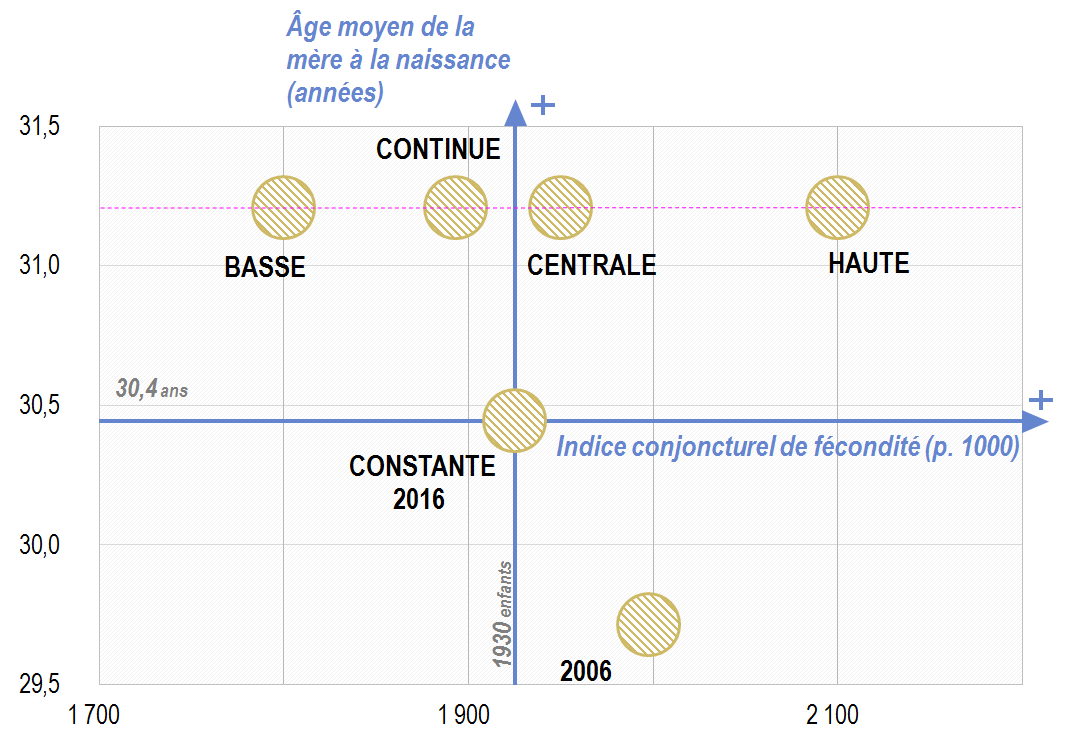
\includegraphics[width=\textwidth]{HYPOFEC}
\caption{Fourchette indicative des niveaux de fécondité à projeter}
\begin{flushright}
\source{Source : INSEE}
\end{flushright}
\end{figure}
\subsubsection{Mortalité}
Etant donné que le suivi est aussi individuel, le quotient de mortalité est une mesure adaptée afin de générer les trajectoires de vie. L'INSEE met à disposition ces quotients de manière régulière au regard des enregistrements de décès mais a également anticipé les évolutions pour les 50 années à venir. Les données sont disponibles par sexe et âge, variables fortement discriminantes. Cependant, d'autres disparités apparaissent et notamment entre les niveaux d'éducation. Etant donné que cette information est disponible avec une fiabilité conséquente, il semblait donc intéressant d'intégrer cette dimension. Les données ne discriminent pas les différents niveaux de diplôme avant les 30 ans, une seule série de quotients est disponible et ce d'une part car les taux de mortalité sont les plus faibles et l'impact est donc minime, d'autre part du fait que les individus n'ont pas encore tous atteint leur niveau d'éducation maximal, certains ont une caractéristique transitoire et donc la mesure finale n'en serait que biaisée. Le choix qui a été fait est donc une combinaison de ces deux contraintes : la tendance globale projetée est utilisée et les disparités inter-diplômes, à chaque âge dès les 30 ans et selon le sexe, sont gardées constantes \textcolor{magenta}{[\ding{89}Table 3.2]}.
\\\\
Ce choix implique toutefois une limite à plus long terme : pour les plus jeunes, un fois que ces derniers atteignent 30 ans, il faut leur attribuer un niveau de diplôme. Mais l'anticipation des répartitions de niveaux de diplômes n'a pas été faite dans ce travail, c'est pourquoi les quotients appliqués sont ceux issus de la tendance centrale. A une échelle de 20 ans cela n'a un impact que limité, puisqu'ils n'atteignent pas encore les âges de mortalité les plus critiques.
\subsubsection{Migrations}
La logique des migrations est quant à elle différente.
Les migrations entrantes sont traitées par une approche plus numérique. C'est à dire qu'un niveau de nouveaux arrivants va être défini, à travers un nombre annuel moyen stable, dans un premier temps du moins. Cette partie est en lien avec la seconde mission [Cf. Chapitre2], puisque c'est au travers de la participation aux études partenariales que la réponse est venue se développer. Cela a permis d'avoir une meilleure compréhension des logiques mobilités résidentielles, en l'occurrence entrantes, avec l'analyse des données de FiDéLI. Les éléments structurants sont en grande partie démographiques, d'autant que les caractéristiques socio-professionnelles ne sont pas traitées dans le simulateur démographique. C'est à dire ce qui distingue les migrations est la notion de cycle de vie.\\
Au regard des observations du fichier de migrations, les profils ont été recrées et ainsi les nouvelles lignes individus répondaient aux contraintes sur les critères que sont : l'âge, le sexe, la taille des ménages, le type de ménage, les diplômes. Ce travail a été fait à partir du fichier des migrations résidentielles à l'année et les nouvelles bases sont constituées sous Excel \textcolor{magenta}{[\ding{89}Figure 3.3]}.\\
Les profils sont regroupés selon 4 groupes, qui correspondent à des regroupements de modalités de la variable TYPMR\footnote{Type de ménage regroupé}[Cf. Table 1.2].\\
Les hypothèses ne sont pas réellement constantes puisque la part de chaque type peut varier, mais en revanche le type d'individu et les âges moyens des types de ménages correspondent aux distributions actuelles.\\
\begin{table}\centering
\begin{tabular}[width=\textwidth]{|l|l|} 
   \hline
    \large{Type} & \large{Modalités de TYPMR} \\
    \hline
    TYP1 & 11, Homme vivant seul\\
    \cline{2-2} 
        & 12, Femme vivant seule\\
	  \hline
    TYP2 & 20, Plusieurs personnes sans famille\\
		\hline
    TYP3 & 31, Famille princ. monoparentale composée d'un homme avec enfant(s)\\
    \cline{2-2} 
        & 32, Famille princ. monoparentale composée d'une femme avec enfant(s)\\						
    \hline
		TYP4 & 41, Famille princ. composée d'un couple de deux actifs ayant un emploi\\
    \cline{2-2} 
        & 42, Famille princ. composée d'un couple où seul un homme est "actif en emploi"\\						
		\cline{2-2} 
        & 43, Famille princ. composée d'un couple où seule une femme est "actif en emploi"\\						
		\cline{2-2} 
        & 44, Famille princ. composée d'un couple d’aucun "actif en emploi"\\	
		\hline
\end{tabular}
\caption{Regroupement effectué sur la variable TYPMR afin de créer les 4 types de profils de nouveaux entrants}
\begin{flushright}
\Source{Source : INSEE}
\end{flushright}
\end{table}
\newpage
\subsection{Visualisation}
La visualisation des résultats dans l'optique d'une version "client" a commencé à être constituée. L'accès au Simulateur Démographique déjà existant n'étant pas possible, les premières sorties se font donc de manière autonome. Cela est consolidé dans une page Html contenant un script php où sont enregistrés les calculs de projection \textcolor{magenta}{[\ding{89}Listing 4.1, Figure 4.2]}.
\\\\On peut y retrouver les tableaux présentant les résultats en fin de période selon une projection initiale avec des hypothèses prédéfinies. Les résultats macroscopiques sont déclinés en nombre d'habitant par année, nombre de ménages et taille moyenne ainsi que le nombre de naissance sur la période, l'âge moyen à chaque 1er janvier.
\\\\Cette évolution du volume global est également représentée par une courbe, elle s'actualise lorsque de nouveaux calculs sont effectués.
\\\\Les éléments de structures sont également présents sous la forme d'une pyramide des âges dynamique. Il s'agit d'un object JavaScript, superposant initialement la première et la dernière représentation des distributions par âge et sexe. Cependant il est possible de changer l'année. Le choix se fait à travers un formulaire html, représenté par un curseur borné, qui renvoie la valeur désirée afin d'uniquement changer l'affichage et non relancer les calculs \textcolor{magenta}{[\ding{89}Listing 4.3]}.
\\\\Faire varier les hypothèses est en l'état possible, mais uniquement à travers l'ICF. Les taux de fécondité par âge gardent la même répartition mais le niveau est recalé sur la valeur envoyée. Cette fois, les calculs sont relancés, c'est à dire que les trajectoires individuelles de l'ensemble des individus sont générées à nouveaux. Ce procédé est donc plus lourd puisqu'il relance le script php et ne modifie donc pas uniquement l'affichage. L'interactivité se fait à travers un procédé AJAX\footnote{Asynchronous JavaScript and XML} et les données sont transmises dans le format JSON\footnote{JavaScript Object Notation}\textcolor{magenta}{[\ding{89}Listing 4.4]}.\\\\
Cette phase relève vraiment de l'exploration puisque je ne connaissais que les rudiments de l'architecture de ces processus. Ce qui m'a permis d'avancer est un schéma explicatif de Loïc présentant les entités nécessaires et les actions qu'elles engendraient. De plus, les nombreux forums en ligne et les tutoriels m'ont permis d'avancer pas à pas, notamment en se réappropriant des codes préconcus et disponibles en open-source. Les sites internet OpenClassroom et StackOverlow m'ont été d'une aide précieuse.
\clearemptydoublepage
\chapter[Etudes sur les migrations résidentielles]{Etudes sur les migrations résidentielles}

\section{Description des partenariats}
L’objectif de ces partenariats est de publier des études statistiques sur des territoires spécifiques tout en approfondissant une problématique qui constitue un enjeu local. En effet, chacune des deux parties apporte son expertise : l’INSEE dispose de données précises et dont l’accès leur est exclusif mais n’est munie d’une connaissance territoriale relativement limitée, ce qui en revanche est un point fort des agences d’urbanisme.
\\\\
Cette collaboration entre la direction régionale Bretagne de l’INSEE et l’AUDIAR a débuté en 2016 et comporte 3 publications. La première traitait des questions de mixité sociale et de pauvreté dans le territoire métropolitain rennais, elle a été publiée en décembre 2016. Par la suite, en février 2017, une seconde étude a porté son attention sur la situation des jeunes adultes, sous-population caractéristique de la métropole rennaise, quant à la formation et l’insertion professionnelle.
\\\\
Dans les deux cas les études ont pu être valorisées auprès de tous les citoyens y portant de l’intérêt, puisque l’INSEE dispose d’une visibilité conséquente, notamment au travers sa collection Insee Analyses - Bretagne. Dans un même temps, elles servent de travaux de référence pour les élus, devenant ainsi des outils d’aide à la décision. Dans une visée rétrospective, de tels travaux permettent également une validation, ou non, des mesures prises sur le terrain économique et social. Bien que discret lors du processus, Rennes Métropole prend part aux comités de pilotage, c’est-à-dire que les différentes versions du travail leur sont soumises et la publication finale nécessite leur validation des messages diffusés.
\\\\
Les équipes de travail du côté de l’INSEE ont changé en fonction de la thématique et de la source de données. Cependant, le procédé reste le même et on retrouve comme contact principal un chef de projet ainsi qu’un technicien. Ce binôme suit le projet de A à Z, dans la réalisation comme dans la communication. Pour autant, tous les messages doivent être validés et ils ne peuvent publier sans l’aval des niveaux hiérarchiques supérieurs.
\\\\
Le procédé est sensiblement symétrique du côté AUDIAR à l’exception que le binôme n’a pas varié entre les publications. Isabelle de Boismenu, sociologue de formation, a été en charge de la coordination des publications tout au long du partenariat. Le traitement quantitatif et les échanges techniques relatifs à la construction des données a davantage été porté par Loïc Bourriquen. Le directeur de l’agence, Henri-Noël Ruiz est lui aussi impliqué, mais principalement sur les orientations et  sur non la construction méthodologique.
\\\\
Dans cette perspective, le troisième volet a débuté dès le mois de mars 2017. L’idée était donc de mettre à profit une nouvelle source de données, le fichier FiDéLI [Cf. Encart] millésimé 2015. Traité de manière conjointe avec la nouvelle version du fichier détail des migrations résidentielles, millésimé 2013, intégrant un laps de temps de 1 an, l’exploitation de la source avait pour objectif de livrer un travail approfondi sur les différentes dynamiques que connait, encore une fois, le territoire métropolitain rennais. L’un permettant d’avoir une idée qualitative, laissant ressortir des causes ou motifs de migrations. L’autre permettant d’objectiver et quantifier les flux. Rapidement le travail a été scindé en deux, donnant lieux à des publications distinctes.
\subsection{Chronologie}
\section{Publication sur les données FiDéLI}
La convention passée entre les deux parties s’était donné un double objectif : 
\\\\\ldots Caractériser les migrations/populations venant façonner chaque zone de la métropole. Cette première partie pouvait difficilement faire état d’évolution des mouvements puisque la source était traitée pour la première fois, il s’agissait donc de tirer un état des lieux en apportant des explications complémentaires aux logiques observables à travers les sources usuelles. Notons que la direction régionale de l’INSEE Bretagne faisait partie des pôles pilotes sur le traitement des données.
\\\\\ldots Observer les migrations intra-communales, ou du moins de manière plus fine en se focalisant sur les QPV\footnote{Quartiers Prioritaires de la Ville}. En l’occurrence l’ensemble de ces derniers se situent dans la ville centre. L’objectif étant de prendre en compte les effets de rétention ou de passage, notamment en comparant différentes sous-populations. Pour quelles raisons quitte-on le logement ? Les réponses peuvent être apportées à différents niveaux [Cf. Encart], tant sur la localisation y compris vers un éventuel autre QPV ou dans une proximité très marquée, sur les évènements familiaux, de nouveaux revenus ou bien du fait politique à travers l’attribution d’un logement social hors de ces limites.
\\\\Ces apports potentiels très riches méritaient chacun une publication propre c’est pourquoi ils font l’objet désormais de deux projets différents. Malheureusement le second point n’a pu être traité dans le temps imparti du fait d’une mauvaise construction de la base de données au niveau national, les premiers traitements ayant donné lieu à trop d’incohérence. Cela peut paraitre étrange étant donné que les migrations relatives à l’échelle infra-communale sont incluses dans le niveau supérieur, mais l’INSEE a assuré que les premiers résultats ne seront pas entachés par ces erreurs sans trop s’épancher sur la question. Ainsi la publication est repoussée en 2018 et fera suite à un premier travail entrepris à l’échelle nationale, voire régionale. La mission présentée occultera donc cette partie.
\\\\Le travail s’est organisé autour de deux grandes instances : les comités techniques, dits « Co-techs », et les comités de pilotage, dits « Co-pils ». Il m’a gracieusement était permis de participer à chacune des rencontres et étapes, ce qui donne une vue complète sur la réalité du travail nécessaire pour aboutir aux fameux « 4 pages ».
\\\\Les comités techniques se sont organisés entre les binômes de chaque partie ; en l’espace de 6 mois, 5 rencontres de ce type ont eu lieu. L’Insee fait une présentation des possibilités d’analyse au regard des données disponibles et les comités permettent de recadrer le champ, notamment grâce à l’expertise de l’AUDIAR. Il s’agit principalement d’un espace d’échange et de réflexion, de proposition méthodologique devant recouvrir au mieux la problématique sociétale.
\\\\Durant ces phases la partie AUDIAR avait surtout pour rôle de mettre en avant les points d'analyse à accentuer et des pistes sur lesquelles creuser. Le principal atout était de donner un territoire qui faisait sens, à travers le découpage territorial. Cette lecture permet ensuite d'avoir une utilité pour les politiques publiques. Certains faits prennent alors sens à travers ces conseils, comme des sur-représentations de flux dans certains cas liés à des livraisons de logements sur l'année concernée.
\\\\La méthodologie utilisée pour traiter des données à multiples dimensions a été la catégorisation par CAH\footnote{Classification Ascendante Hiérarchique}. Les résultats les plus déterminants dans les motifs de migrations étaient les évènements liés aux cycles de vie, et c'est sur cet axe qu'ont été développés les traitements. La source de donnée fait également ressortir principalement cette dimension, bien qu'elle soit marquée, car les variables économiques sont relativement peu détaillées. Dans cette optique là il a donc été intéressant pour moi de prendre part puisque cela correspondait relativement bien aux compétences développées dans le master, et ainsi je n'ai pas été cantonnée à la seule observation de ces rendez-vous. Comme prévu dans le plan initial, cela a été un élément décisif dans les choix relatifs aux migrations pour le simulateur.
\\\\Ce travail technique est soumis de manière plus espacée aux comités de pilotage, en l’occurrence 2 fois sur la période, avec les autres acteurs comme définis ci-dessus. La formulation des termes y est revue mais également la mise en avant ou retrait de certains points ressortant des traitements de données. La dénomination des classes est un des points qui ont été discutés, afin d'éviter et on peut ainsi voire que les termes statistiques et politiques ne sont pas tout à fait identiques.
\\\\La rédaction a été en très grande partie faite par l'INSEE et il est assez difficile d'intervenir sur le produit final, ce qui est parfois un peu frustrant. A mon sens, le rendu est très numérique alors que les résultats ont une portée plus qualitative, les proportions par exemple ne pouvant pas être directement comparées avec les sources de données classiques du fait de leur unité statistique particulière que sont les migrations. Le seul prisme comparatif intéressant serait à faire dans le temps, mais les publications à fréquence annuelle ne sont pas prévues ou bien avec d'autres territoires comparables, ce qui n'est actuellement pas le cas.
\\\\La publication est pour l'instant en cours de formatage dans les services d'infographie désormais externes à l'INSEE. Elle sera à partir d'octobre 2017 accessible en ligne à la suite d'une sortie coordonnée avec l'étude présentée ci-après lors d'une conférence de presse.
\boitemagique{Fichier démographique sur les logements et les individus, FIDELI}{
Cette base de données constituée par l’Insee se base sur les déclarations fiscales.
\\\\
L’\textbf{atout} majeur de ces données est l’enregistrement continu de la situation l’entité fiscale, permettant en partie un suivi longitudinal contrairement au recensement qui se positionne dans une approche transversale.
De plus, la localisation est très fine « au carreau » permettant un traitement inter mais également intra-communal.
\\\\
Dans la perspective des migrations résidentielles, on peut identifier les foyers fiscaux ayant connu un changement d’adresse ou non. Ainsi on peut identifier des motifs ayant conduit à une modification résidentielle par la comparaison des caractéristiques pré et post migrations. De fait, un millésime d’année N relate les évènements étant intervenus lors de l’année N-1.
Bien que les interprétations partent d'analyse statistiques et non déclarative, différents axes sont identifiés comme motifs générant une migration résidentielle :
\\\ldots Les évènements familiaux : Décohabitations, séparations, veuvage ...
\\\ldots Les changements de type de logement : Passage en logement plus grand, plus petit...
\\\ldots Les changements socio-économiques : Entrée/sortie en logement social, survenu de précarité, acquisition d'un bien, amélioration des revenus globaux ...
\\\ldots Les changements géographiques : Passage en péri-urbain, ville centre, aire urbaine, QPV, changement de région
\\\\
\textbf{Précautions} : L’unité de travail est la migration, différente de l’individu, mais également du ménage. Les résultats ne sont donc pas immédiatement comparables avec les sources usuelles.
\\\\
Pour autant cette source comporte également des lacunes constituant des \textbf{limites} à l’analyse :\\
\\\ldots La notion de foyer fiscal diffère de celle de ménage : deux ménages peuvent former un même foyer et la réciproque est également vérifiée. Les faits démographiques sont donc déformés être peuvent être corrigés au cas par cas tant les réalités des ménages sont variables.
\\\ldots La couverture est de mauvaise qualité chez les jeunes adultes, souvent étudiants. Cela a d’autant plus d’impact sur cette étude que cette tranche d’âge constitue une part essentielle des migrations.
}
\newpage
\section{Publication sur les données du Recensement}
Cette publication est quant à elle publiée au nom de l’AUDIAR, bien qu’elle vienne s’inscrire en complément de l’étude précédente\textcolor{magenta}{[\ding{89}pp70-94]}. Cette fois la dimension technique au sens de construction des données est donc à la charge de l’agence d’urbanisme. Il s’agit de dresser un tableau complet de la question des migrations résidentielles. La principale différence est donc une contrainte moindre en termes de volume de contenu, mais devant apporter des chiffres précis afin d’objectiver les tendances ressenties et dont les mesures précises se font rares concernant la métropole.
\\\\Comme il l’a déjà été évoqué, Loïc Bourriquen a régulièrement été absent durant cette période et ainsi le travail avec Isabelle de Boismenu est devenu de plus en plus conséquent.
\subsection{Processus \& Organisation du travail}
Les objectifs initiaux étaient clairs mais laissaient toutefois une grande marge de manœuvre. Il a fallu dresser un état des lieux sur les migrations résidentielles posant avant tout les grandes lignes sur les bases du fichier détails des migrations. Pour le reste, cette publication devait être complémentaire à celle issue du partenariat.
La première phase à consister à cibler la sous-population d’étude, en l’occurrence l’ensemble des individus ayant transité par Rennes Métropole, c'est-à-dire détenant le code commune d’une des 43 entités lors de l’année de recensement OU (inclusif) lors de l’année antérieure. Concrètement la table comporte XXXXXXX lignes ainsi que l’ensemble des variables du fichier et est supposée représentée plus de 480 000 individus.
\\\\Ensuite, afin d’identifier les profils de migrations, ce qui correspond au cœur de l’étude, les individus ont été classés en 5 catégories, au regard des comparaisons entre lieu de résidence actuel et lieu de résidence antérieur déclaré [Cf. Table 2.1].
\newpage
\begin{table}
\begin{tabular}{ | l | p{12cm}| }
 \hline \large{Profil} & \large{Description} \\
 \hline Stable & \small{N’a connu aucun changement de logement et réside dans RM}\\
 \hline Entrant & \small{Ne résidait pas dans RM auparavant, réside dans RM désormais}  \\
 \hline Sortant & \small{Résidait dans RM auparavant, ne réside plus dans RM désormais}\\
 \hline Mobile\_RM & \small{Résidait dans RM, réside désormais dans une autre commune de RM}\\
 \hline Mobile\_COM\_RM & \small{Résidait dans RM, réside toujours dans cette même commune mais a changé de logement en 2012}\\ \hline
 \end{tabular}
\caption{Description des différents profils de migrations utilisés}
\end{table}
\\\\De même, il a fallu déterminer des zonages, regroupant les nombreuses communes, tant dans RM qu’en dehors [Cf. Table 2.2].
\\\\ \textit{Nb : Passé le cœur de métropole, la distinction est parfois faite entre les 4 points cardinaux dans l’analyse afin de différencier les zones lors que les logiques ne sont pas homogènes.}
\renewcommand{\arraystretch}{1.5}
\begin{table}
\begin{tabular}{| l | p{11cm} |}
\hline \large{Entité géographique} &  \large{Description} \\
\cline{1-2}
\multicolumn{2}{|l|}{\large{\textit{Découpage intra-communal}}} \\
\hline \ldots Rennes & Capitale régionale et principale ville de la métropole \\
\hline \ldots Cœur de Métropole & Communes adjacentes 4 \\
\hline \ldots Pôles structurants & Communes ayant un poids et des infrastructures conséquentes \\
\hline \ldots Autres communes & Autres communes non incluses dans les catégories ci-dessus \\
\cline{1-2}
\multicolumn{2}{|l|}{\large{\textit{Découpage supra-communal}}} \\
\hline \ldots Aire urbaine & Communes incluses dans l’aire urbaine de Rennes comme définie par l’INSEE en 2010, hormis les communes de RM \\
\hline \ldots Proximité & Le reste de l’Ille et Vilaine, ainsi que les départements directement adjacents \\
\hline \ldots Grand Ouest & \\
\hline \ldots Ile de France & Ensemble des 8 départements d’ile de France \\
\hline \ldots France entière & Ensemble des autres communes françaises, métropolitaines et ultra-marines, non incluses dans les catégories précédentes \\
\hline \ldots Etranger & Modalité présente uniquement pour les entrants, car seuls les individus recensés sur le sol français sont présents dans la base. Les départs vers l’étranger peuvent être approximés par déduction dans l’équation démographique générale ; il est cependant impossible de connaitre leur lieu de départ ainsi que leurs caractéristiques socio-démographiques \\
\hline
 \end{tabular}
\caption{Description des différents zonages utilisés}
\end{table}
\begin{figure}\centering
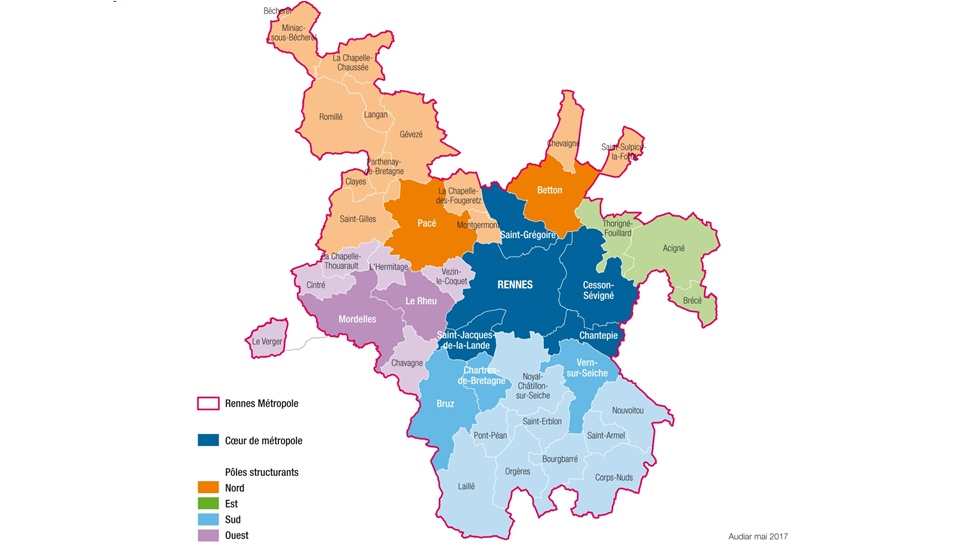
\includegraphics[width=\textwidth]{CARTOZONAGE}
\caption{Représentation cartographie des zonages utilisés lors de la publication sur les migrations résidentielles}
\begin{flushright}
\source{Source : AUDIAR}
\end{flushright}
\end{figure}
\\\\Une fois les éléments décrits mis en place, les approches se sont faites en allant de données de cadrage à des données précises. Les échanges ont été très interessants et ont permis se poser des questions. Le travail s’est donc structuré sous forme de navette entre la réalisation d'objets statistiques et la lecture du phénomène [Cf. Figure 2.2]. Les approches sociologiques et statistiques se sont complétées tout au long du travail, puisque la faisabilité à travers les données conditionnait les résultats possibles mais ces derniers devaient apporter des réponses à la réalité de la métropole et de ses logiques.
\begin{figure}\centering
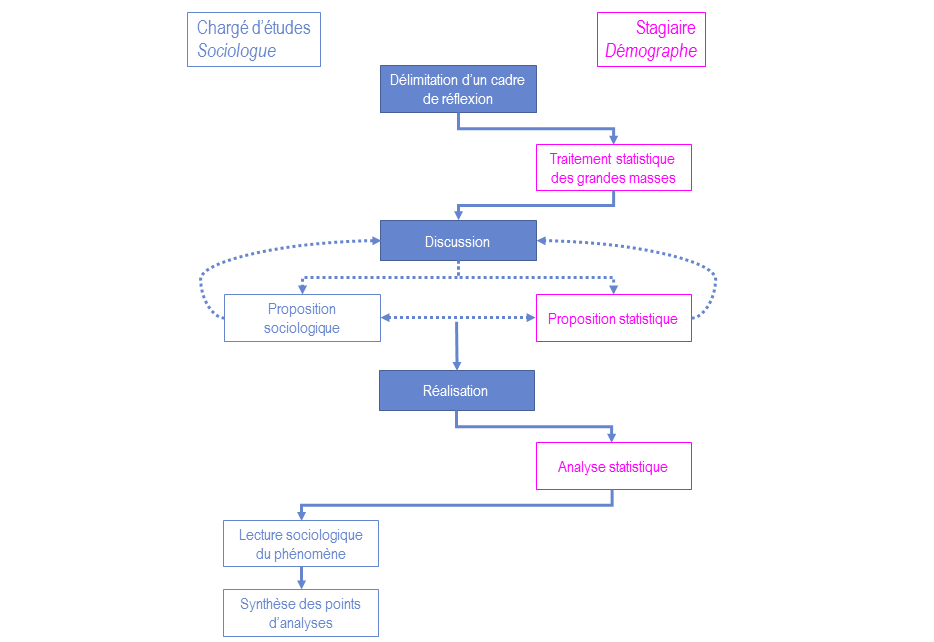
\includegraphics[width=\textwidth]{ORGAMISSION2.png}
\caption{Schéma d'organisation de travail lors de la publication sur les migrations résidentielles.}
\end{figure}
\\\\Le plan de l'étude dans sa version finale la publication est découpé en 3 grandes parties :
\begin{itemize}
\newpage
	\item Données de cadrage,		\textit{Partie I}
	\item Logiques spécifiques à chaque profil,		\textit{Partie II}
	\item Impact territorial de ces mouvements,		\textit{Partie III}
\end{itemize}
\subsection{Méthodologie de travail}
Les méthodes de traitements sont plutôt basiques, c'est-à-dire que la quasi-intégralité des résultats sont issus de statistiques bivariées. L’environnement de travail est inclus dans Excel qui est l’environnement habituel de traitement de données pour les chargés d’études à l’AUDIAR. En effet pour faire le travail de navette avec Isabelle, sociologue de formation, cet environnement est plus facile d’accès que le logiciel R, très peu usité dans l’agence mais également avec le service infographie qui peut se l’approprier plus aisément lors de la mise en page. Des statistiques plus complexes, multivariées, auraient pu être entreprises mais la lecture des résultats est plus compliquée et cela n’était pas nécessaire étant donné le public est large et les résultats se veulent accessibles au plus grand nombre.
\\\\Ainsi le travail consistait principalement à cibler les populations concernées par les différents points d’analyse pour présenter des mesures qui font sens et également à proposer des indicateurs pertinents, voire originaux.
\\\\L’adaptation des représentations à ces différentes mesures faisait également partis du travail entrepris, qu’il s’agisse de graphiques, tableaux ou bien cartographies. Ces dernières ont été traitées grâce au logiciel QGis.
\subsection{Difficultés rencontrées}
La première version de la base a connu un soucis lors de la réimportation et ainsi la vérification initiale a laissé passer des erreurs, ce qui a amené à recommencer cette étape. Pour autant les premiers travaux entrepris n’étaient pas sans utilité, ils ont notamment permis d’entrevoir les incohérences et les traitements potentiels.
\subsection{Choix effectués}
Dans cette partie sont présentés les choix relatifs et les raisons ayant motivé ces constructions statistiques; la rédaction finale peut parfois diverger de ce qui est écrit.
\subsubsection{Partie I : Grandes masses}
Le premier traitement a été de poser les bases démographiques en repartant de l'équation générale, c'est à dire les composantes naturelles et migratoires. Il était important de considérer les mouvements internes puisque leur impact sociologique sur le territoire n'est pas sans effet et que les trajectoires résidentielles se font souvent par rebond, une installation n'étant pas définitive. En 2013, $16\% $ des individus occupaient leur logement pour la première fois.
\\\\Etant donné que le recensement ne se focalise que sur les communes de résidence de l’année N-1 et N, il parait à première vue difficile de savoir si les individus ont un lien de longue date avec le territoire. Pour autant l’effet du retour au pays est un élément qui revient souvent. Le traitement des départements de naissance permet d’approcher la question bien que cela ne relate qu’une situation initiale et non des durées de présence dans les zones concernées. Seules les personnes de référence du ménage et leur éventuel conjoint été pris en compte dans cette analyse s’alignant ainsi sur l’hypothèse que dans un cadre familial les enfants ne pèsent pas dans le choix de cet effet retour.
\\\\ Les destinations des sortants sont présentés à travers les grandes modalités définies et ici on peut observer que beaucoup d'individus restent dans les alentours de la métropole. D'une part, bons nombres d'entre eux se dirigent vers l'aire urbaine. Cette proportion conséquente diminue nettement lorsqu'on se focalise sur les ménages, puisqu'il s'agit en grande partir d'installations familiales dans des zones pavillonnaires plus accessibles économiquement et correspondant à un désir de cadre de vie. De même, le grand ouest a un poids non négligeable et trouve en partie pour moteur le retour des étudiants arrivés dans la ville centre quelques années auparavant du fait de l'attractivité régionale des pôles universitaires; ces explications prennent d'autant plus sens avec la première étude partenariale.
\subsubsection{Partie II : Différentes logiques de mobilité}
L'objectif de cette partie a été de prendre en compte les singularités de chaque profil de migrations et pour cela il est toujours interessant de les comparer à la structure des 'stables'.
\\\\Le premier traitement a donc été fait sur l'âge qui est une composante non-négligeable. Dans cette étape j'ai proposé de basculer l'âge par année étant donné que les amplitudes classes n'étaient pas identiques. Le choix des courbes a été fait pour une meilleure superposition. Les apports de cette analyse sont nombreux et on peut constater que les jeunes adultes sont les moteurs de ces mouvements, dans un sens comme dans l'autre puisqu'ils représentent les parts les plus importantes. On peut aisément supposer que le passage est de rigueur plus que l'installation de long terme étant donné un décalage assez net des entrées et sorties du système. Les jeunes parents ne semblent pas statiques puisque les enfants sont relativement mobiles et ne peuvent migrer de manière autonome. On constate d'ailleurs que les migrations dans Rennes Métropole sont sur-représentées entre 30 et 40 ans. Pour autant, une fois ce seuil passé, les changements de logement sont de plus en plus rares. Un évènement apparait toutefois, il s'agit des départs de Rennes Métropole qui connaissent un pic juste après 60ans, âge auquel on peut associer le départ en retraite.
\\\\La distribution des niveaux de diplôme selon le profil de migration est également un élément intéressant; dans un premier temps il a fallu ôter tous les individus non concernés, c'est à dire ayant moins de 15ans. Ces résultats s'ils sont lus de manière rapide alarment parfois les décisionnaires en remettant en cause la capacité de Rennes à attirer des personnes diplômées. En effet, les diplômés du supérieur sont structurellement plus importants du côté des départs que des arrivées. Or on constate que déjà chez les néo-rennais leur niveau de diplôme est plus important que la structure initiale du territoire car en effet les étudiants sont attirés par la ville, mais connaissant également un retour une fois leur formation terminée. Entre temps leur condition face au diplôme a évoluée.
En effet, bon nombre d’individus issus de la région parisienne ayant déjà travailler sont référencés en tant que cadres et professions supérieures et à contrario la part de CSP\footnote{Catégorie Socio-Profesionnelle} autres est plus faibles, l’hypothèse sous-jacente est que les étudiants franciliens sont relativement peu nombreux à venir se former dans la capitale bretonne. Ces proportions ont tendance à s’inverser dans les départements de proximité, où les offres de formation sont souvent moindres et de fait empiète sur les cadres. Pour autant, la manne de ces CSP supérieures, enjeux réel d’attractivité, provient d’avantage du Grand ouest. C’est pourquoi il semblait plus intéressant de présenter les résultat par CSP plutôt que par territoire afin de porter l’analyse sur un angle différent du discours ambiant.
\\\\
En revanche, les taux de chômage pour les franciliens s’inscrit dans la logique de la distance à la métropole : plus le lieux d’origine est éloigné, plus le taux de chômage est conséquent. Cela semblait allait à l’encontre de travaux antérieurs, c'est-à-dire qu’il semblait contre-intuitif de penser que des populations plus précaires faisaient un déménagement d’aussi longue portée dans la métropole. Comme il l’a récemment été mis en avant, les fichiers détails permettent de considérer le chômeur autrement qu’un 'Robinson isolé' \footnote{Anatomie sociale de la France: ce que les big data disent de nous, Hervé le Bras, 2016} grâce à la situation du ménage de l’individu. C’est pourquoi un focus sur les couples permet de voir que la part de couple dont un actif en emploi cohabite avec un actif sans emploi est importante, ce qui peut être perçu comme un effet de liane : un conjoint trouve dans un premier temps un travail, le ménage change de territoire et se réimplante dans l’emploi par la suite. L’Ile de France est sur-représentée dans cette combinaison ce qui peut apporter un élément d’explication à ce taux de chômage relativement élevé.
\subsubsection{Partie III : Effets territoriaux}
Ici, l'unité de travail pertinente est apparu être le ménage à travers les caractéristiques de la personne de référence puisque les polarisations se focalisent principalement sur les distinctions socio-économiques; il semble donc inutile de prendre en compte les enfants des familles par exemple. Les variables disponibles dans la source de données sont assez limitées et on retrouve principalement la CSP. Le niveau de diplôme peut permettre une approximation mais les effets de génération peuvent venir masquer les réelles variations de capital économique, les anciens étant généralement moins diplômés. De même, la catégorie des retraités est traitée de manière uniforme dans la déclinaison des CSP bien que l'hétérogénéité des profils soit conséquente. De même, le postulat associant monoparentalité et niveau de vie peu élevé n'est que partiellement vérifié pour le territoire rennais, comme il l'a récemment été mis en avant. C'est pourquoi cette partie constitue un éclairage nécessaire et tout à fait fiable mais mériterait d'être recoupée avec d'autres éléments.
\\\\La troisième partie de la publication a voulu mettre l’accent sur les effets de migrations sur les territoires et d’éventuels effets de polarisation. Les migrations des plus précaires sont à priori régulées par les politiques locales d’habitat. Les contraintes de logement sociaux ont été fortes dans chaque commune de la métropole et de plus ces programmes sont censés se répartir au mieux sur le territoire afin justement d’éviter de créer des zones trop déséquilibrées en termes de niveaux de vie et socio-professionnels. C’est pourquoi mettre l’accent sur la ségrégation par le haut ou choisie, c'est-à-dire concernant les migrations des ménages les plus favorisés, semblait être plus important. Les cartographies associées permettent de visualiser ces différentes dynamiques à travers la représentation des modalités considérées comme les plus élevées, à la fois sur le diplôme mais également les CSP.
\\\\
Les résultats ne sont pas si nets et l'échéance annuelle ne peut permettre d'affirmer des tendances lourdes. La deuxième couronne de Rennes semble toutefois entamé une mutation avec une attractivité auprès des publics jeunes et socialement aisés, particulièrement au sud. L'Ouest quant à lui est plus à la peine. La distinction entre première couronne nord et sud s'accentue quelque peu.
\\\\La distinction des âges présentées comme telles est à mon sens biaisée puisque les classes ont été faites à la main sans garantir une réelle homogénéité interne afin de ne pas pointer du doigt certaines communes.
\\\\Seule cette partie présente des résultats à la commune, mais certains effectifs vraiment trop faibles, n'ont pas été représentés car leur fiabilité est compromise.
\subsection{Freins et difficultés surmontés}
Un des points auxquels il a fallu prêter attention est de se détacher quelques peu des stéréotypes que chacun a en tête sur ces questions et de ne pas abonder systématiquement dans ce sens.\\\\
Il était également nécessaires de prendre certaines précautions dans la lecture des résultats puisqu’il s’agit d’une année précise et donc les variations peuvent être liés à des évènements conjoncturels, du type sortie d’un parc de logement ou bien ouverture de logements sociaux. Même si les éléments présentés sont légendés, les données étant relatives à 2012, cela peut contribuer à des images déformées des sociologies communales. C’est pourquoi il faut essayer de capter des tendances un peu plus lourdes que la variation annuelle. Un zonage un peu grossier permet de passer outre ce phénomène et ainsi les résultats sont lissés avec le regroupement, ce qui laisserait toutefois penser que ces entités sont homogènes. Dans un même temps, l’intérêt de la publication était aussi de voir s’il y avait des endroits spécifiques, il a donc fallu trouver le bon équilibre.
\\\\L’hypothèse selon laquelle le logement neuf entrainerait des mobilités a fait partie des points abordés lors des discussions. Cette problématique relative à l'ancienneté du bâti a été difficile à traiter du fait du mode de collecte du recensement. Le croisement entre profil de migration et ancienneté du logement a mis cette incohérence en avant puisque les individus considérés comme stables durant l’année 2012 présentaient des taux de logements construits après 2011 trop conséquents. L’explication peut probablement résider dans le décalage entre millésime et année réelle de collecte, variable d’une commune à l’autre. C'est-à-dire qu’au sein du millésime 2013, faisant état des mouvements opérés en 2012, sont présents des individus recensés entre 2011 et 2015. Par exemple :\\
Un individu/ménage ayant changé de logement durant 2013 et recensé en 2015 affirme habiter dans la même logement que l’année précédente (2014); son logement actuel est neuf, donc après 2011, ce qui est vrai. Il est ainsi considéré comme stable dans un logement tout récent, d'où l'incohérence.\\\\
\ldots Option 1 : Retrouver l’année de construction de son logement précédent, \textit{impossible}\\
\ldots Option 2 : Distinguer les modalités : par bonds de 2 ans pour les emménagements récents, et couvre 5 ans pour l’ancienneté des logements.\\
\ldots Option 3 : Présenter les résultats tels quels, \textit{trop incohérent}\\
\ldots Option 4 : Ne pas présenter, ce qui a été choisi.
\\\\\\En dehors ce des points techniques, je n'ai pas ressenti de difficultés particulières étant donné que j'intervenais en tant que support. Les seules contraintes étaient davantage d'ordre organisationnel puisque nos congés ne coïncidaient pas; il a fallu valider les tâches faites en autonomie à la fin de l'été afin de pouvoir boucler la publication et de la coordonner avec les travaux de l'INSEE qui a également fait des relectures dans le cadre du partenariat.
\clearemptydoublepage
\part[Bilan \& Perspectives]{Bilan \& Perspectives}
\chapter[Evaluation \& Analyse personnelle]{Evaluation \& Analyse personnelle}
\subsection{Apports en termes de Savoir-être}
Plusieurs aptitudes ont pu être mobilisées ou tester durant ces deniers mois.\\
\ldots\textit{Aptitudes dans le projet}\\
Au-delà même des éléments pertubateurs, la méthode de travail attribuée au Simulateur m'a appris à travailler de manière autonome et c'est là le principal point de ce stage. Dans la perspective des objectifs, j'ai donc du apprendre à penser des des solutions, à conceptualiser, organiser et délimiter un cadre de travail. Bien sûr cela relève encore de l'apprentissage et il y avait malgrè tout des limites prédéfinies puisque Loïc est responsable du projet. Dès le début j'avais été mise ne garde sur l'dffet boomrang que peut avoir à posteriori une erreur en début de chaine et j'ai donc porté attention à ce point mais également j'ai aussi pu le comprendre à mes dépens.\\\\
\ldots\textit{Autres aptitudes}\\
La prise d'initiative a de fait découler de cette approche. J'ai donc du apprendre à faire preuve de lucidité et tenter d'évaluer l'interêt que peut avoir telle ou telle piste, mesurer le gain potentiel et la perte de temps que cela peut egendrer, ce qui n'est pas toujours évident.\\Cette experience, et particulièrement les imprévus, m'a amenée à être perseverante mais également à rebondir en passant à autre chose, et il n'est pas toujours évident de trouver le point de bascule.
\subsection{Apports en termes de Savoir-faire}
Les compétences techniques mises à l'épreuve ont été multiples durant cette immersion professionnelle. On peut toutefois les distinguer sur plusieurs plans :\\\\
\ldots\textit{Nouvelles compétences}\\
La majeure partie d'entre elles relèvent du champs de la programmation informatique avec la découverte des languages JavaScript et des processus d'interaction amenant à des résultats dynamiques.\\La modélisation à travers des nombres aléatoires, référant aux méthodes dites de Monte-Carlo, ont pu être approchées mais pour autant cela a principalement relevé de l'experimentation que d'un vrai cadre théorique.\\
Parallèlement au projet, j'ai décidé d'apprendre à rédiger du contenu en LaTex afin de pouvoir améliorer la qualité de rendus papier mais également informatiques à travers l'intégration de formules mathématiques, difficilement gérable autrement. Mais surtout, l'idée était de ne pas être tributaire des licences Mirosoft ou Adobe notamment à titre personnel, puisque LaTeX est libre et gratuit.\\\\
\ldots\textit{Compétences développées}\\
Dans le champs de la programmation toujours, j'ai pu réutiliser les interrogations de bases de données via le language SQL, des processus d'automatisation de traitement en php et des sorties html, comme appris durant la première partie de mon cursus universitaire. L'environnement du serveur WAMP était alors un souvenir lointain mais désormais je me sens familière grâce à l'utilisation répétée des commandes de bases.\\
L'utilisation de R a également été élargie à de nouveaux usages dans la gestion des données mais également dans la capacité à valoriser les travaux et les méthodes de travail grâce aux notebooks.\\La découverte du package Qgis2Map m'a permis de valoriser différemment le travail cartographique.\\\\
\ldots\textit{Compétences consolidées}\\
Le traitement de base de données, en particulier du recensement, et la valorisation des phénomènes longtemps traités de manières théoriques ont pris une dimension conrète. Leur représentation catograhphiée a pu être mis à contribution. L'utilisation de ces compétences est devenue fluide à force de répétitions.
\subsection{Adéquation entre formation \& missions de stage}
Dans l’ensemble la formation reçue à l’IDUS était vraiment en très bonne adéquation avec la structure et en discutant avec les différents salariés ils trouvaient que le profil développé en formation de démographie était très interessant.
\\Les points forts :
\begin{itemize}
	\item Polyvalence importante entre traitement et analyse et donc un degré d’autonomie étant donné que la donnée prend beaucoup de place dans les travaux.
	\item La maitrise des outils cartographiques est une compétence très appréciée.
	\item La connaissance approfondie des sources de données publiques notamment, de la constructions aux biais induits dans l'analyse.\\
\end{itemize}
Les aspects à developper :
\begin{itemize}
	\item Les projections de population sont des connaissances assez recherchées mais les méthodes apprises lors du master limitent assez rapidement. Il n’est pas nécessaire de toutes les approfondir mais au moins de donner des clefs pour aller chercher d’autres pistes.
	\item L'utilisation de serveurs de données externes permettant de gérer des bases plus conséquentes et expliquer comment est organisé un ordinateur.
	\item Une approche un peu plus algorithmique, dans R par exemple, pour apprendre à bien créer des fonctions basiques avec les logiques de boucle, ce qui permettrait de gagner beaucoup de temps en TD mais aussi en travaillant.
\end{itemize}
\subsection{Propositions non retenues}
J’ai grandement apprécié le degré de liberté et autonomie qui m’ont été attribué lors de ce stage, mis à part les turbulences. J’ai pu faire bons nombres de proposition et la feuille de route n’a jamais été figée. La dialogue a été très enrichissant, et les propositions que j’ai pu soumettre ont toujours été écoutées, souvent retravaillées et sont présentes dans les éléments présentés auparavant.\\
Un seul des éléments soumis n’a pas été repris. Il s’agit d’une version web des données sur les migrations résidentielles. L’objectif était de mettre à disposition un ensemble de données difficilement représentables dans une publication papier ; il s’agissait dans ce cas d’un diagramme de Chord représentant les échanges de flux migratoires entre les différents zonages. Au début j’ai effectué cette représentation en m’inspirant d’une version proposée par l’APUR\footnote{Atelier Parisien d'URbanisme}, juste pour essayer, et j’ai vu l’intérêt suscité chez mes collègues non statisticiens qui trouvaient ça « amusant », mais beaucoup moins lorsqu’ils voyaient mes feuilles de calcul infinies. C’est pourquoi l’intérêt était double,  d’une part rendre plus attrayante les informations et donc amener les lecteurs à parcourir la publication, d’autant plus que la diffusion des études se fait également en ligne et en particulier sur twitter ; mais également de mettre à disposition un niveau de détails plus important où chacun peut y trouver son compte selon la zone d’intérêt. Mes collègues étaient partants mais les différentes contraintes de chacun ont fait que cela n’a pas été, pour l’instant, mis en place. La version de ce travail n’est donc pas finalisée mais toute l’architecture est là. Il s’agit d’une page html dont les données visualisables sont intégrées au script, ce qui est plus facile d’utilisation qu’une référence à une tiers base sur serveur, type phpMyAdmin\textcolor{magenta}{[\ding{89}Listing 5.1, Figures 5.1, 5.2]}.
Une cartographie avec les zonages est également juxtaposée à ce diagramme et est issue de QGis, puis exportée grâce à l’extension Qgis2Map. L’objectif final était de mettre en surbrillance les résultats d’une modalité lors du survol avec curseur sur la carte mais je n’ai continué.
\clearemptydoublepage
\chapter{Conclusion \& Perspectives}
Les enseignements de ce stage sont nombreux et m’ont largement éclairée pour les décisions professionnelles qui m’attendent. J’ai trouvé les réponses à mes interrogations tant dans les apprentissages techniques, les relations humaines mais également les divers disfonctionnements auxquels j’ai été confrontée.
\\\\Le premier point concerne avant tout une mise en garde sur les choix concernant le bien-être entreprise. Il m'a paru important de détenir une expertise, certes, sur le sujet de travail mais de toujours rester en mesure de rebondir si les conditions de travail ne sont pas satisfaisantes. C'est pourquoi garder la capacité de changer d'entreprise m'est apparue comme un élément très important, ce qui peut devenir difficile lorsque le travail est trop spécifique à un domaine.
Les méthodes de management ne sont pas un point que j'ai développé mais j'ai pris conscience qu'elles étaient essentielles puisque les relations humaines constituent une part fondementale dans la cohésion des équipes de travail et donc de la qualité du travail entrepris. 
\\\\Ensuite je dirais qu’il m’a paru important d’être vraiment à jour sur les outils de traitement de données dans le côté statistique du démographe. C'est-à-dire que les évolutions méthodologiques sont très rapides et qu’une fois en entreprise il est beaucoup plus difficile de rattraper les wagons ou bien d’entreprendre une pause formation en milieu de carrière.
\\\\En parallèle j’ai senti que j’avais la curiosité et le d’apprendre de nouvelles méthodes car le travail de chargé d’études statistiques peut être, ans la technique et non sur le fond, assez répétitif. La mise à disposition de nombreuses sources de données est vraiment une chance à mon avis et il est parfois frustrant de se sentir limitée par le manque de connaissance ou à minima de ne pas savoir où trouver les outils potentiels et connaitre le champs des possibles, notamment grâce aux rudiments de certains langages informatiques.
\\\\De plus, j’ai aimé l’aspect ingénierie entrepris lors de la première mission davantage que le côté rédactionnel et mise en synthèse des résultats. J’ai vraiment été séduite par l’idée de développer un outils comme le simulateur démographique et plus largement des supports spécifiques pour l'évaluation et la prospective.
\\\\C’est pourquoi j’ai décidé de postuler à l’Ecole Nationale de la Statistique et l’Analyse de l’Information, Bruz, au sein d’un master spécialisé intitulé Smart Data pour une durée d’un an. Ce que j’ai apprécié dans l’offre de formation sont la rapidité et l’intensité du cursus, l’ouverture à l’international ainsi que l’utilisation exclusive de l’anglais mais surtout, à la différence des autres formations en science de la données, c’est la forte identité de la statistique publique puisque sont formés dans le même établissement les futurs analystes de l’INSEE.
\\\\Ensuite j’ai vraiment apprécié la taille de la structure qui permet d’avoir une diversité importante dans les profils des salariés mais également une proximité avec ses collègues. L’organisation en projets était très intéressante et permet de travailler tour à tour avec des individualités différentes. L’ouverture à des acteurs de territoire est aussi très enrichissante comme cela a été le cas avec l’INSEE mais également les élus ou bien des observatoires de problématiques connexes. Bien que ça n’est pas était tout à fait le cas dans les projets auxquels j’ai participé j’apprécie grandement l’utilité qu’ont les travaux de l’agence d’urbanisme dans l’organisation quotidienne du territoire et donc des habitants, dans les alertes véhiculées lors des analyses mais également du travail réflexif sur les politiques publiques.
\\\\C’est pourquoi je pense dans un premier temps m’orienter vers des expériences me permettant de développer le côté innovant du métier. Pour autant j’aimerais vraiment contribuer, à terme, à des projets ayant une utilité plus sociétale que commerciale comme les agences d'urbanisme par exemple le propose. Dans cette optique ce stage de fin d'études a vraiment été fondateur et m'a permis de choisir une orientation pour la suite.
\clearemptydoublepage
\backmatter
\clearemptydoublepage
\addcontentsline{toc}{part}{Sommaire détaillé}
\tableofcontents
\newpage
\addcontentsline{toc}{part}{Liste des tableaux}
\listoftables
\newpage

\end{document}